\documentclass[final,leqno,onefignum,onetabnum]{siamltexmm}
\usepackage{amsmath}
\usepackage{color,graphicx} 

\title{Detecting Hand movements from EEG Signals\thanks{Kaggle Grasp and lift competition. 
\url{https://www.kaggle.com/c/grasp-and-lift-eeg-detection}}} 

\author{Anirudhan J Rajagopalan, Michele Cer\'u\thanks{New York University (\email{ajr619@nyu.edu}; \email{mc3784@nyu.edu}). Questions, comments, or corrections to this document may be directed to this email address.}}

\begin{document}
\maketitle

\begin{abstract}
  This project aims to detect and classify the grasp and lift hand movements of a subject from EEG (Electroencephalography) recordings.
  Successful identification and classification of the recordings will help in developing Brain Computer Interfaces (BCI) that can be used to restore the ability of patients to do day-to-day tasks.
  We are provided with \~24 series of grasp and lift actions performed by twelve subjects.  We run our models using the first \~18 series as our training and the last \~2 series as our test set.
  We use the level1 predictions of the Kaggle contest winners as our baseline and try to compare the performance of our model against the level1 predictions of baseline.
  Using our simple pipeline we are able to show that we can get accuracy of 0.61 Mean Area Under the Curve (MAUC)\@.
\end{abstract}

\section{Introduction}

Electroencephalography (EEG) is used to record electrical activity of the brain.
It is typically noninvasive, with the electrodes placed along the scalp.  
In the Grasp And Lift (GAL) experiment twelve subjects were asked to perform lifting series in which the object's weight (165, 330, or 660g), surface friction (sandpaper, suede, or silk surface), or both, were changed unpredictably between trials, thus enforcing changes in fingertip force coordination.\cite{naturegal}
The hand movement of the subject was recorded by 3D sensors which were synchronized with the EEG cap thus providing us with the exact moment at which the GAL events happen.  With respecct to our goal of classifying the hand movements, we have to detect the following six events.

\begin{enumerate} 
  \item \textit{HandStart}: Beginning of the movement.
  \item \textit{FirstDigitTouch}: Making contact with the object.  
  \item \textit{BothStartLoadPhase}: Starting to load the object. 
  \item \textit{LiftOff}: Holding the object up.
  \item \textit{Replace}: Replacing the object in its original position.
  \item \textit{BothReleased}: Releasing the fingers from the object. 
\end{enumerate}

The EEG signals recorded by 32 electrodes fixed to the scalp are recorded at a frequency of 500Hz.  An added objective of this task is to make sure that we dont use any future data for doing predictions (No future data rule, as described in the data page of the challenge).  This restriction is imposed to mimic the real life scenarios in which such an application can be used, wherein, we will not have access to any of the future data while making predictions in real life.\cite{website:kaggle-competition}


This project aims to classify the hand movements of subjects by using EEG signal data.  We compare the performance of LinearSVM and GaussianSVM combined with VLAD and Bag of Features (BOF) feature representations.  We base our performance using the Area Under the Curve as described in the Kaggle challenge.  We try to reason the performance of our model with respect to the dataset by analysing the spatial relationship and variance of the features.  We then discuss about models that we might use to tackle this hard problem.

\section{Dataset Description}

\subsection{Sources and Format}
The dataset is provided by Kaggle Inc.\ for their Grasp and Lift Detection challenge\cite{website:kaggle-competition} sponsored by Way Consoritum\cite{website:way_consoritum}.  
The dataset consists of separate test and train zip files of size 153 MB and 915 MB respectively.  
The dataset expands to 447 MB and 3.1GB after extraction.  
Out of these datafiles, we cannot use the testset as they are being used for the competition submissions.  
The testset has only the *\_data.csv files with no corresponding *\_events.csv file.  
Since there is no *\_events.csv file we will not be able to learn or evaluate the performance of our models by using the test dataset provided in the challenge website.
So our effective usable dataset is only the training data which we partition into train and test set for training our models.

The dataset consists of two types of files: 
\begin{enumerate}
  \item{data.csv} --- CSV of series labels and values from the 32 electrode signals.
  \item{event.csv} --- CSV of series labels and event values.
\end{enumerate}
The sample dataset is included below for reference.

\begin{figure}[ht!]
  \centering
  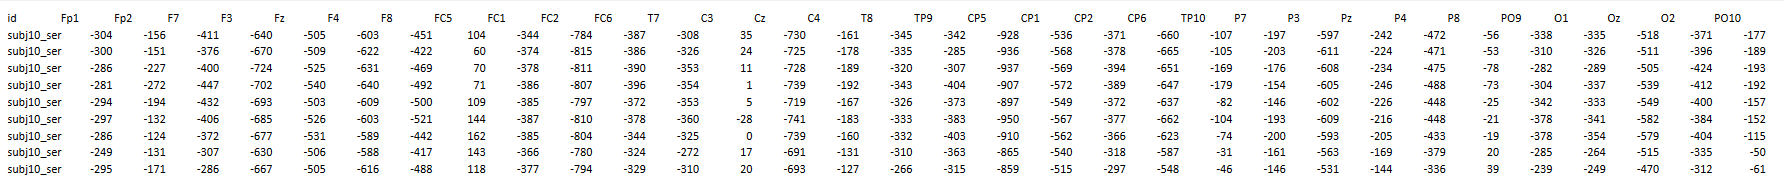
\includegraphics[width=1\textwidth]{images/sample_data}
  \caption{Sample Data format.  The columns correspond to id,  Fp1, Fp2, F7, F3, Fz, F4, F8, FC5, FC1, FC2, FC6, T7, C3, Cz, C4, T8, TP9, CP5, CP1, CP2, CP6, TP10, P7, P3, Pz, P4, P8, PO9, O1, Oz, O2, PO10.\label{fig:Sample_data}}
\end{figure}

\begin{figure}[ht!]
  \centering
  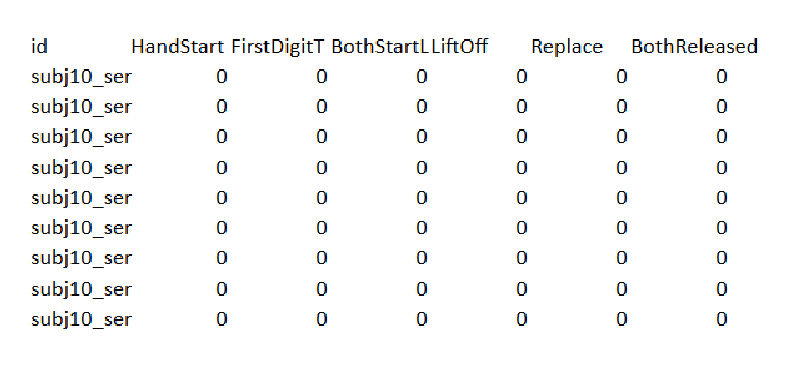
\includegraphics[width=0.5\textwidth]{images/sample_events}
  \caption{Sample Event format. The columns correspond to id, HandStart, FirstDigitTouch, BothStartLoadPhase, LiftOff, Replace, BothReleased\label{fig:sample_events}}
\end{figure}

The event dataset will have a value of 1 corresponding to the event (stimulus) that is being performed at the instant of sampling.  There can be situations where there are multiple stimulus being triggered for the same EEG signal.  The objective is to classify (or) label the input EEG signals to the corresponding stimulus.

The total number of samples across the complete dataset is 17985850.

The spatial relationship between each of the 32 electrodes is given by Fig.~\ref{fig:eeg_spatial_relation}

\begin{figure}
  \centering
  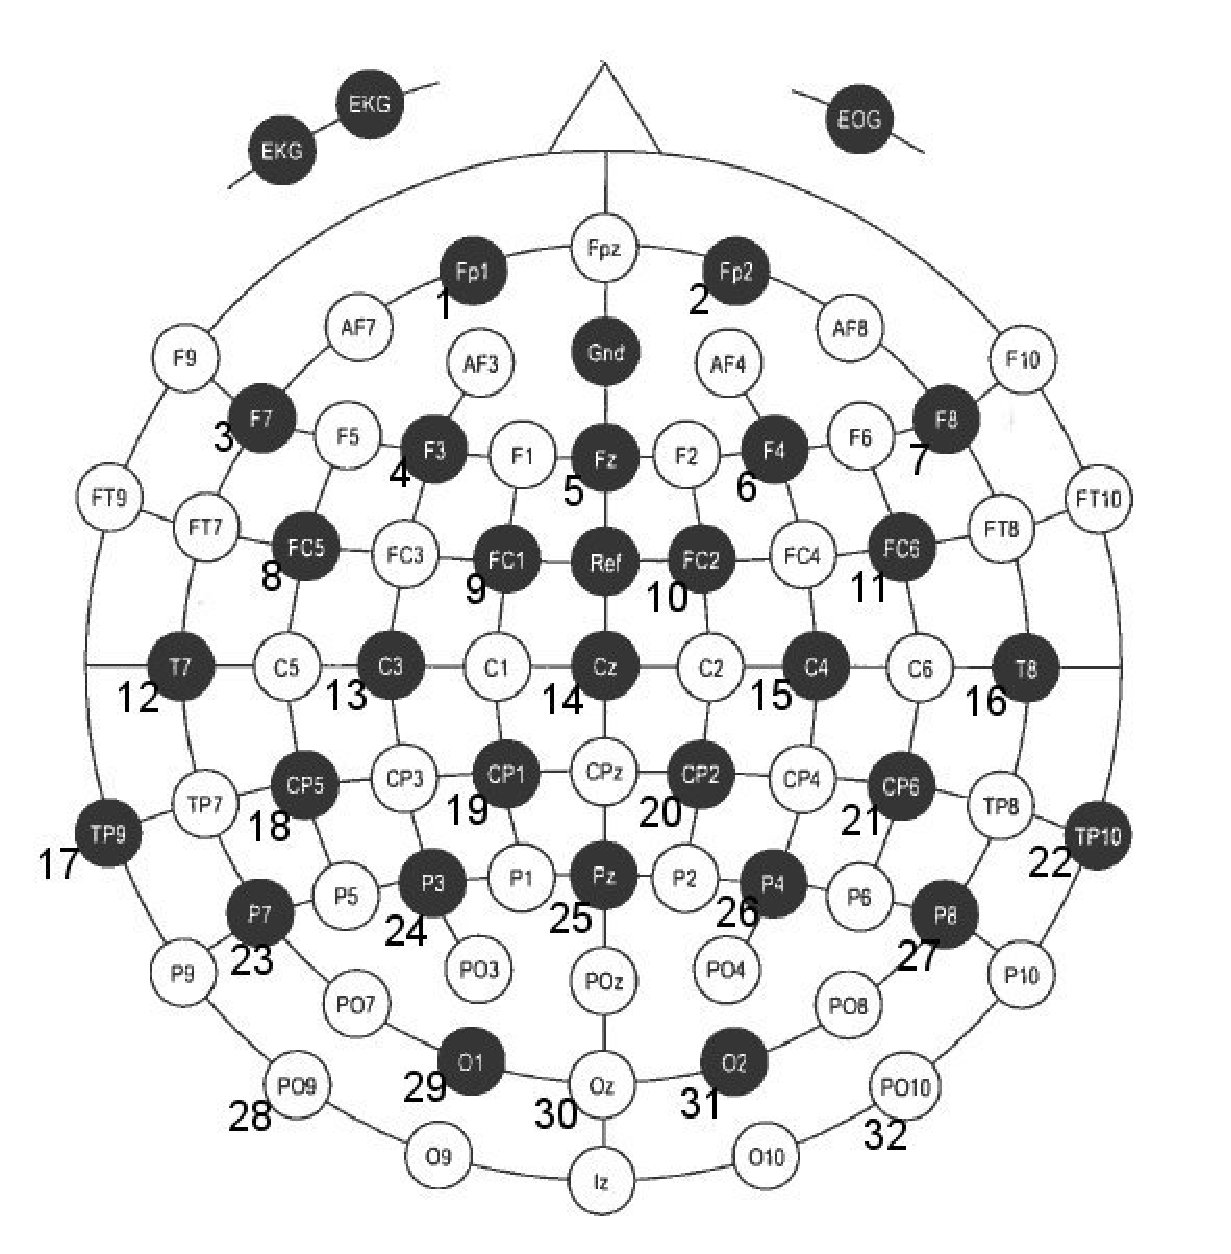
\includegraphics[width=0.5\textwidth]{images/eeg_spatial}
  \caption{Spatial relationship between 32 electrodes.\label{fig:eeg_spatial_relation}} 
\end{figure}

\subsection{Multilabeling or Multiclass classification}
The dataset can have multiple stimulus at the same time as shown in figure~\ref{fig:label_or_class}.
This is an important feature to consider as it forms the distinction between multiclass and multilabel classification problem.
\begin{figure}[ht!]
  \centering
  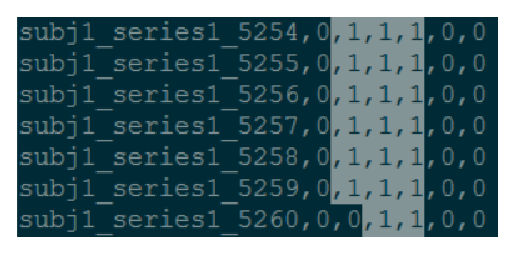
\includegraphics[width=0.5\textwidth]{images/multilabels}
  \caption{Multilabel or Multiclass classification problem.\label{fig:label_or_class}}
\end{figure}

\section{Problem Statement}
As described in the previous section, the objective is to classify/label the input EEG signals with their correspoinding stimulus.  
This is an inherently multilabel classification problem.  
We can reduce this to multiclass classification problem by considering the fact that the events happen in sequence.  
For example, BothReleased event is always followed by Replace which is always followed by LiftOff and so on and so forth.
Thus the problem of finding all events corresponding to the EEG signal can be decomposed into the problem of finding the start of the occurance of a particular event.

The constraint defined above simplifies our problem into a multiclass classification problem.  With proper feature selection and model selection we should be able to solve the problem effectively.

\section{Baseline}
\subsection{Choosing a baseline}
We considered the models developed by Alexandre Barachant (a.k.a cat) and Rafal Cycon (a.k.a Dog) for our baseline model (Cat \& Dog solution)\cite{website:cat_dog_solution}.  
The solution by Cat and Dog won the first prize in the challenge and it makes logical sense to use that as our baseline.   
The cat and Dog solution has three levels of models.


The first level of models uses 

\begin{enumerate}
  \item Covariance Matrices
  \item Event Related Potentials (ERP)
  \item Filter Banks
\end{enumerate}

The solution uses an ensemble of multiple learning models such as Logistic Regression with LDA, Convolutional Neural Network, and Recurrent Neural Networks.  
This model fits our requirement to be a baseline and hence we choose the Level-1 model of \textit{Cat and Dog solution} as our baseline models.
We decided to compare the performance of the baselilne with respect to our own model.
The accuracy achieved by the Level-1 models are not readily available.  So we tried to run the baseline to get the accuracy values.

\subsection{Running the baseline}
The hardware specs listed in the \textit{Cat and Dog solution} page, details the hardware used and the time taken for the entire pipeline.  
Considering that we are using only the Level-1 models as our baseline, we decided to try running the baseline to get a accurate idea of time and performance for Level-1 alone.

\subsubsection{Attempt 1}
We first attempted to run the Level-1 models in our own machines just to get an idea of how much memory and time requirements the Level-1 took.
We started out by installing all the packages specified in the requirements document and then started with the preprocessing step.
The preprocessing step ran successfully even in our local machine and created two numpy binary files \textit{infos\_val.npy} and \textit{infos\_test.npy}.
The numpy files are to be consumed by the baseline files for building the models.


We ran the baseline using \textit{lvl1/genAll.sh} in our local.  The baseline crashed due to out of memory.  Thus we decided to run all our experiments in New York University (NYU)'s High Performance Computing (HPC) clusters\cite{website:nyuhpc}.


\subsubsection{Attempt 2}
The second attempt\cite{website:attempt_2} involved trying to run the Level-1 code using NYU HPC clusters.
\begin{enumerate}
  \item As used in the first attempt, we decided to treat the baseline as a blackbox and try to run the baseline code.
  \item We identified out the entry point for the baseline models and decided to run the model in NYU HPC clusters.
  \item We figured out the modules required to make all the python packages used in the baseline to work and loaded the modules.
  \item We submitted a HPC job for running the baseline.  The job requested for the exact number of CPU nodes, CPU cores, GPU resource and RAM mentioned in the Hardware specs. 
\end{enumerate}

The second attempt to run the baseline also ended without success as the system crased due to mismatch between required packages and the available packages in HPC\@.

\subsubsection{Attempt 3}
Since running the baseline on HPC crashed and running the models on our local resulted in `out of memory' error, we decided to run the baseline in our local using a fraction of the sample.

\begin{enumerate}
  \item We started out by trimming the input files from 18 series of GAL to just 6 series of GAL per subject.
  \item This corresponds to just \~4000 lines of samples per input file and we were able to load the data in our local effectively.
  \item We installed the exact version (including the minor versions) of almost all the packages specified in the baseline.
  \item A few packages that were mentioned in the baseline were not available due to some unknown reason and we had to install the previous version for these packages.
  \item We ran the baseline with the subsample of the original dataset.
\end{enumerate}

We still ran into a number of issues while running the code.  Our guess is that the code in the \textit{Cat and Dog Solution}'s repository has got some breaking changes after the final submission.  We emailed the authors regarding the issue and even after help from the authors we were unable to get the baseline running.

\subsection{Baseline Results}
As discussed above, since we couldn't get the baseline running even after 3 attempts and the help of the authors and since we had spent more than 2 weeks on this problem, we decided to move ahead with building our own solution to this interesting problem.


The attempt to run the baseline gave us significant insights into the Domain, data and assumptions that can be used for solving the problem.

\section{Building our own Pipeline}

\subsection{Understanding the domain}
The biggest challenge for building the pipeline was to understand the domain and figure out the preprocessing tasks.  
The components downstream the pipeline was already fixed to be VLAD\cite{art:vlad_aggregate_paper}\cite{art:all_about_vlad}  and Bag of Features.
After a bit of exploring and a bit of guidance from our professor we decided to use MNE\cite{website:mne_python} for the data preprocessing.  MNE provided us with a number of tools for preprocessing the data.
\begin{enumerate}
  \item Epochs
  \item Covariance measures
  \item XDawn filter\cite{art:Xdawn_filter}
  \item Algorithms to process the raw data and generate the Event Related Potentials.
\end{enumerate}
We made good and extensive use of the codebase of \textit{Cat and Dog} solution to understand the type of preprocessing that was carried out by them.  
We also went through the forum of the Kaggle challenge to gather insight about the domain and ways of processing the data.


\subsection{Data Preprocessing}

We used MNE to consume the raw data in csv format to find the epoch values and the Event Related Potentials.  
We also use MNE to get the covariance matrix on the complete training/test dataset.  
This information is then fed to xDawn filter with WINDOW size as 500.  
The value of the parameter num\_components for xDawn, which determines the number of features in the processed data was varied from 2 to 4 and the resulting three dimensional array was saved in numpy binary formats.

The total run time for data preprocessing took around an hour for the dataset.

\subsection{Exploring the preprocessed data}
We then set out to explore the processed data to better understand the dataset.
\subsubsection{Clustering of local descriptors}
The total number of stimulus that has to be classified is six.  
Any classification task becomes easier if we find that the data is separable by some degree.  
Since our model essentially depends on builing over the clusters formed by local descriptors, we decided to cluster the data to find if there is any amount of separatbility of data.

We ran experiments to cluster the local descriptors for one subject (Subject 1 in the dataset) using MiniBatchKMeans algorithm.  
We then used the cluster information and different markers to plot the cluster information on a two dimensional plot by reducing the dimensionality.
The plot generated for n\_components = 2 is shown as an example in Fig~\ref{fig:local_descriptors_clusters}.

\begin{figure}
  \centering
  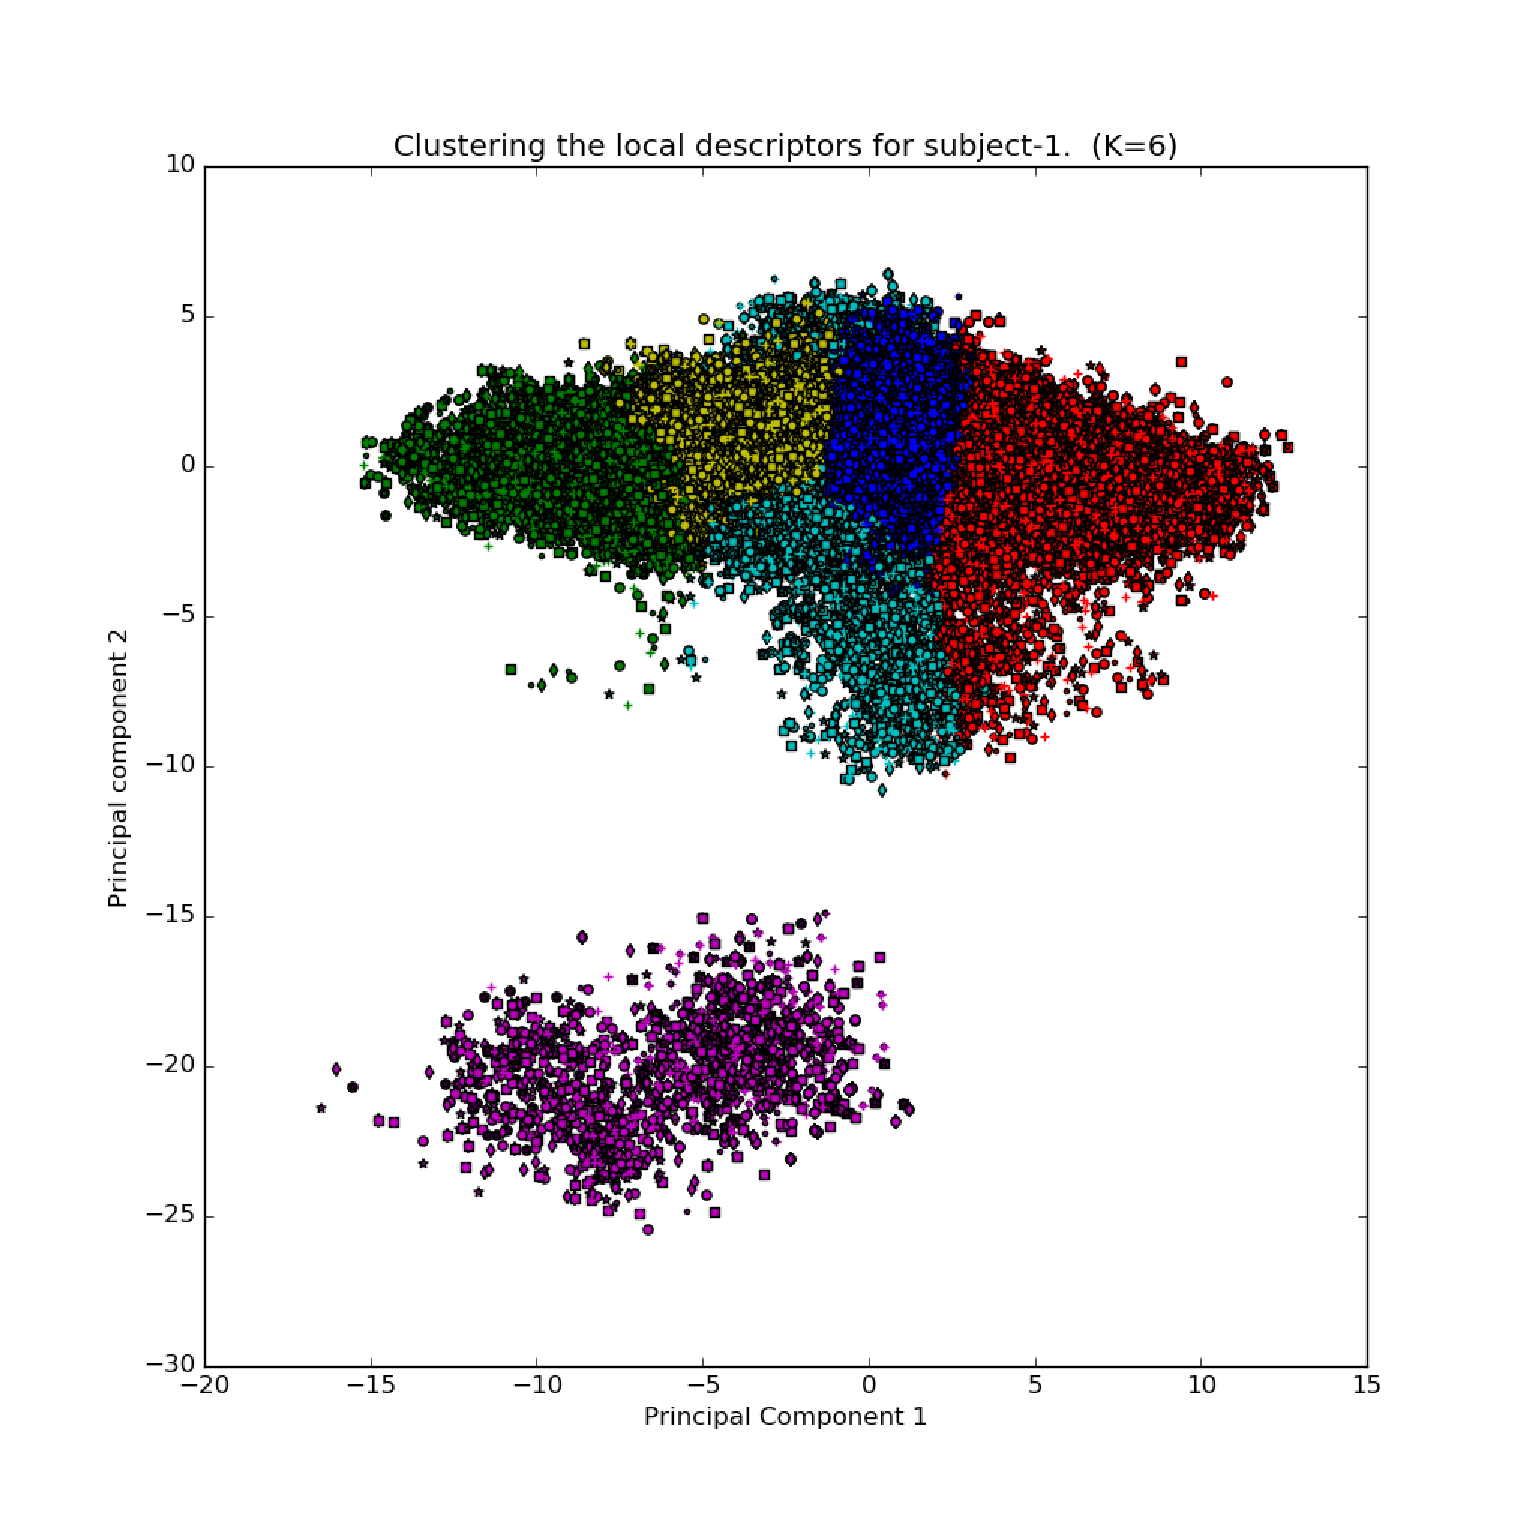
\includegraphics[width=0.75\textwidth]{images/cluster_centers}
  \caption{Clustering the local descriptors of a single subject into 6 clusters.  Different clusters are represented by different colors.  The local descriptors that gives raise to a particular stimulus are denoted by different markers such as plus, star, circle, square and so on.  Just a cursory look on the clusters makes it clear that the data is not separable easily.\label{fig:local_descriptors_clusters}} 
\end{figure}

\subsubsection{Variance of local descripitors}
PCA is a technique for dimensionality reduction.  
It works by finding components that provide the maximum variance (It can be thought of as the direciton in which the features spread out the most).
Finding the variance of the features helps us to understand how the data is spread and how much dimensions we should use to tackle the learning problem.  
We created a plot of the variance of a the local descriptors for a subsample of the dataset (Subject 1).  
The variance curve is as shown in Fig~\ref{fig:ld_variance}

\begin{figure}
  \centering
  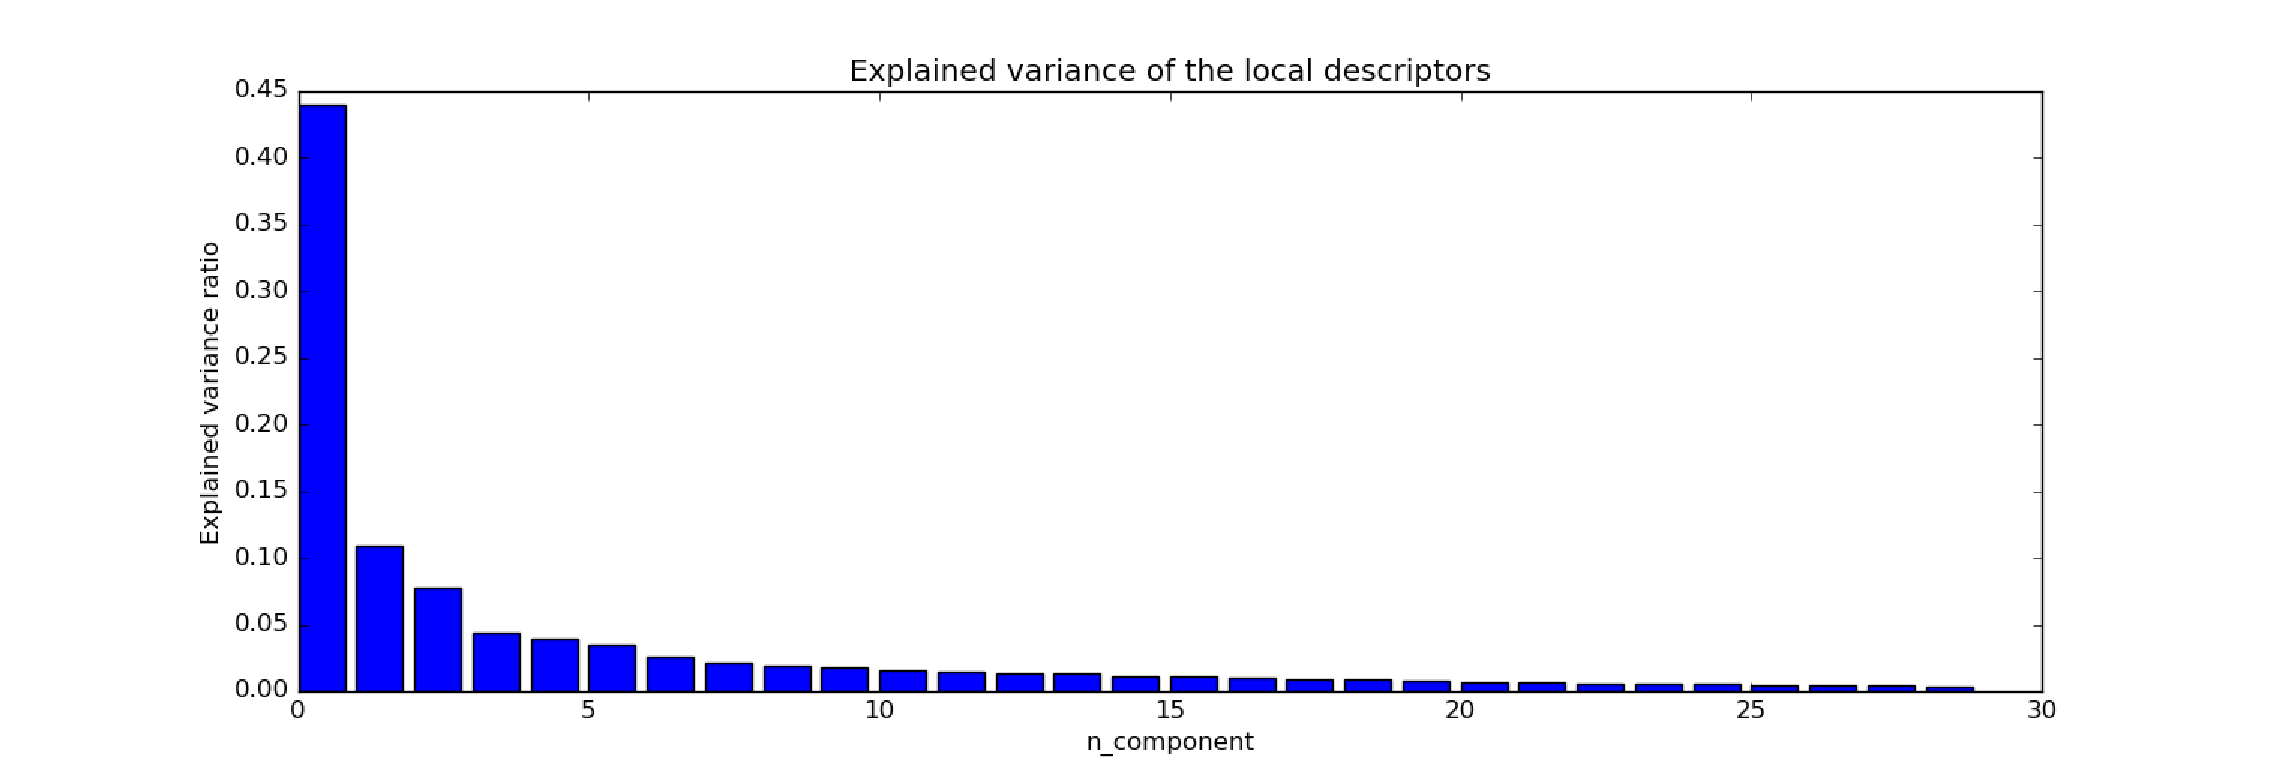
\includegraphics[width=0.75\textwidth]{images/ld_variance}
  \caption{Explained variance ratio of local descriptors for a subsample (Subject 1).  We get variance measures of 99, 95, 90, 77, 65 and 50 for components 29, 21, 16, 7, 4, 2 respectively.\label{fig:ld_variance}} 
\end{figure}

The analysis of variance was actually performed after we got the results for BOF and Vlad models.  This makes us wonder whether the model's performance might have increased if we had used PCA on the local descriptors before applying our models.

\subsection{Building Bag of Words model}
\subsubsection{Theory}
Bag of words feature representation is a way of representing a sample that can be separated into its local descriptors.  
We learn the vocabulary of the dataset using Kmeans with different cluster sizes.
The vocabulary for a learning problem is the cluster centroids found by Kmeans.
We process our data again to find how many local descriptors belong to a particular centroid.
By belong, we denote the centroid that is closest to a particular local descriptor of a sample.
The sample can then be represented as a vector of dimension equal to the cluster size K with the magnitude of each dimension equal to the number of local descriptors belonging to that particular centroid.

\subsubsection{Algorithm}
The following algorithm enumerates the steps for finding the Bow representation of a sample.
\begin{enumerate}
  \item Learn the Codebook $ C = \{c_{1}, c_{2} \ldots c_{k}\} $ of words representing the vocabulary of the domain.
  \item Assign the vocabulary for every local descriptor by $ c_{i} = NN(x) $.
  \item The bow representation is given by the sum of local descriptors belonging to a particular word $ c_{i} $.
\end{enumerate}

Thus we get the BOW representation by the simple formula
\begin{align*}
  B_{j} = \sum_{x \mid NN(x) = c_{j};  \forall j \in K} 1
\end{align*}

\subsubsection{Implementation}
The code for this project is developed using Scikit-Learn\cite{website:sklearn}.  So we wanted to build an implementation that fits well into scikit-learn's pipelines.
Any component can be duck typed to fit into scikit-learn's pipeline if it has fit, transform, set\_params and get\_params methods.  A brief explanation of the methods and its functions is discussed below.
\begin{description}
  \item{def fit (X, Y=None)}  This function is used to learn the parameters from the distribution of the training set and apply the parameters on training and test set.  In our BOW case, this involves learning the vocabulary of the local descriptors.
  \item{def transform (X)}  This function transforms the training/test input by using the vocabulary learnt during the fit method.  In BOW implementation a sample containing a list of local descriptors is transformed into a vector of dimension K (cluster size).
  \item{def set\_params (**params)} Used to set the parameters for grid search.
  \item{def get\_params (deep=True)} Used to get the current parameters.
\end{description}

\subsubsection{Performance}
We try to understand the performance of our Bag of Words implementation by plotting the runtime and memory usage against a fixed number of clustersFig~\ref{fig:bowf_time_fixed_cluster},~\ref{fig:bowf_memory_fixed_cluster} and also against fixed sample sizes. Refer Fig~\ref{fig:bowf_time_fixed_sample},~\ref{fig:bowf_memory_fixed_sample}.
\begin{figure}
  \centering
  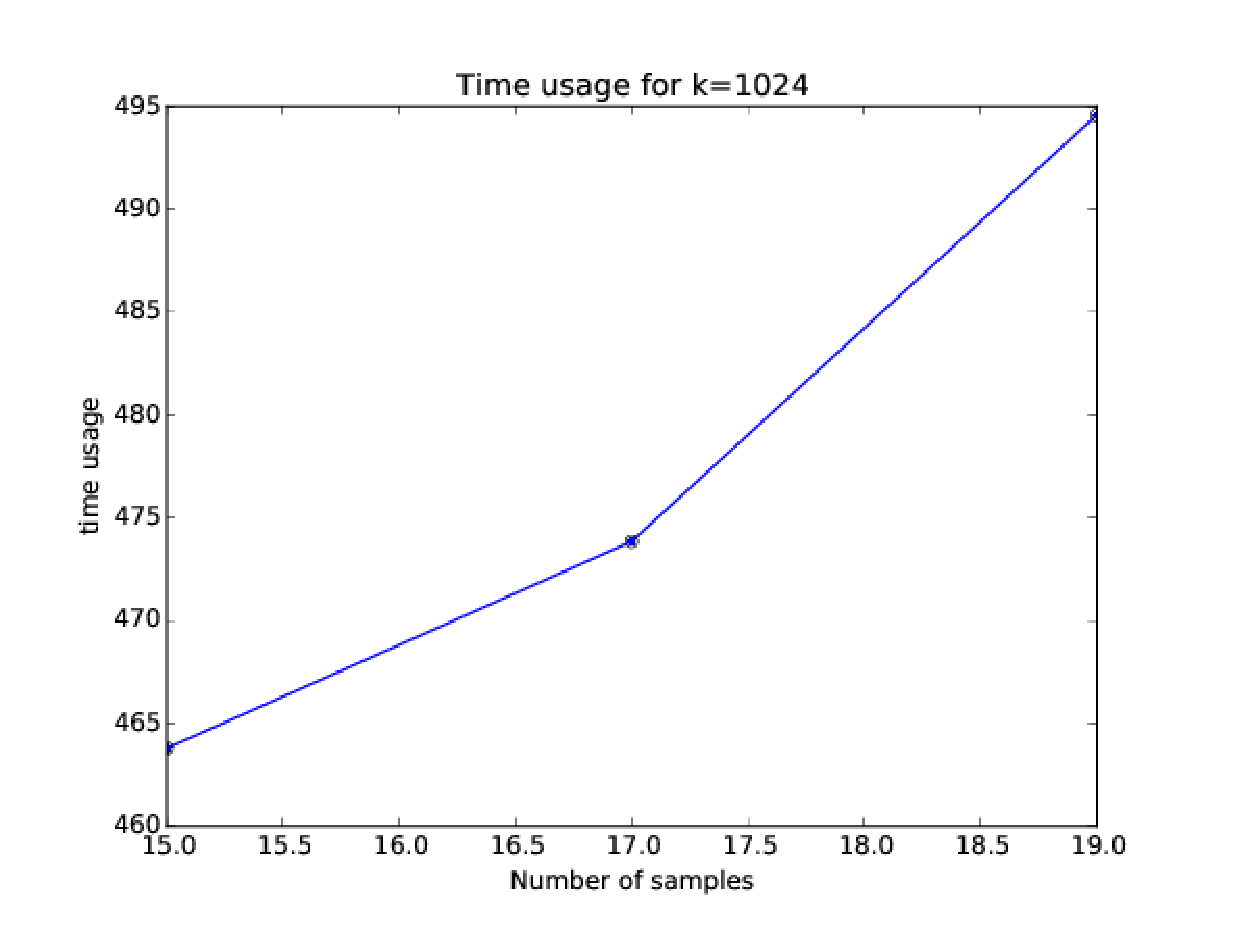
\includegraphics[width=0.60\linewidth]{images/bofwTimeFixedCluster}
  \caption{Bag of Words feature representation: Runtime with fixed cluster size. (Cluster size in $\log_{2}$).  The experiments are run on the actual project dataset.\label{fig:bowf_time_fixed_cluster}}
\end{figure}
\begin{figure}
  \centering
  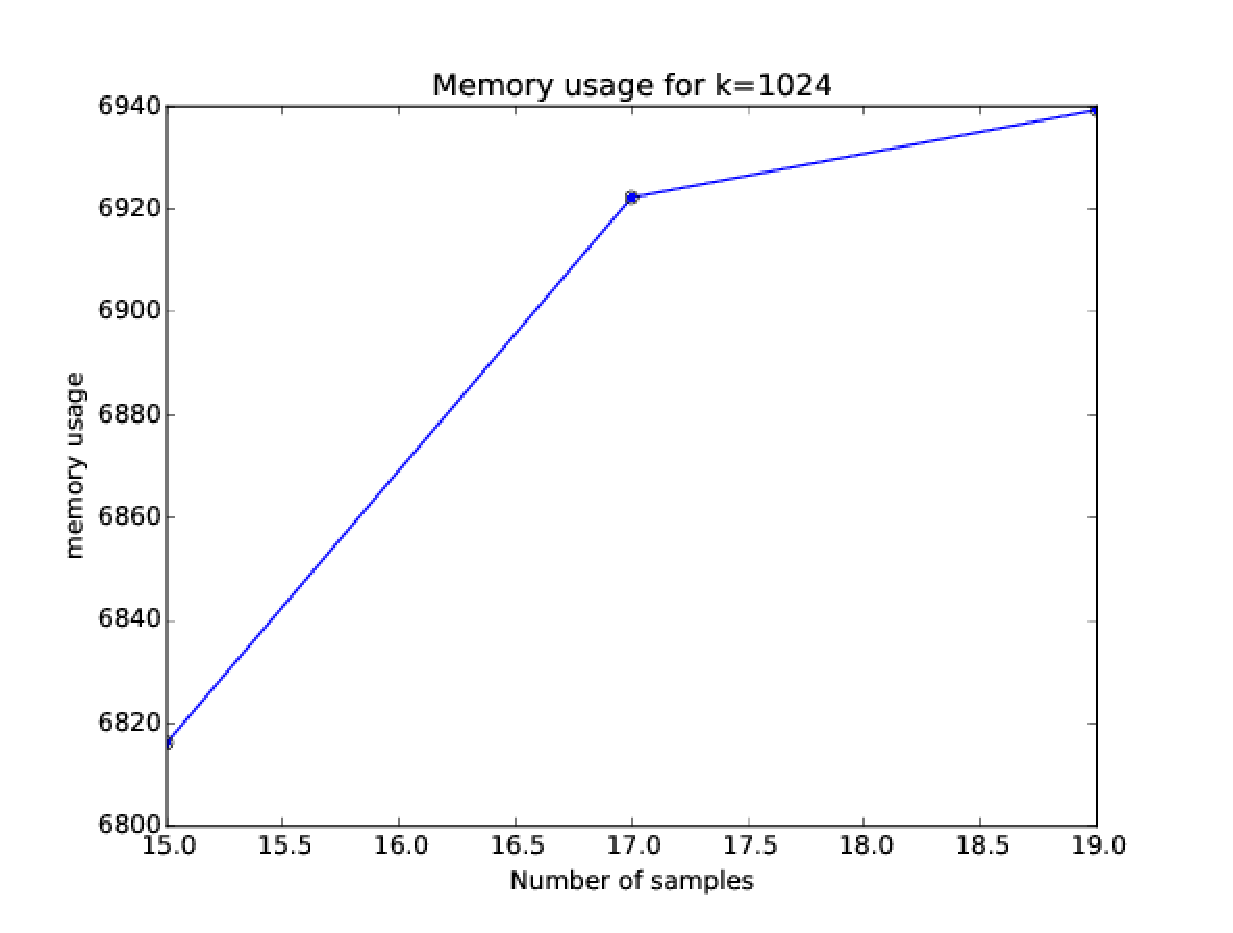
\includegraphics[width=0.60\linewidth]{images/bofwMemoryFixedCluster}
  \caption{Bag of Words feature representation: Memory usage with fixed cluster size. (Cluster size in $\log_{2}$). The experiments are run on the actual project dataset.\label{fig:bowf_memory_fixed_cluster}}
\end{figure}

\begin{figure}
  \centering
  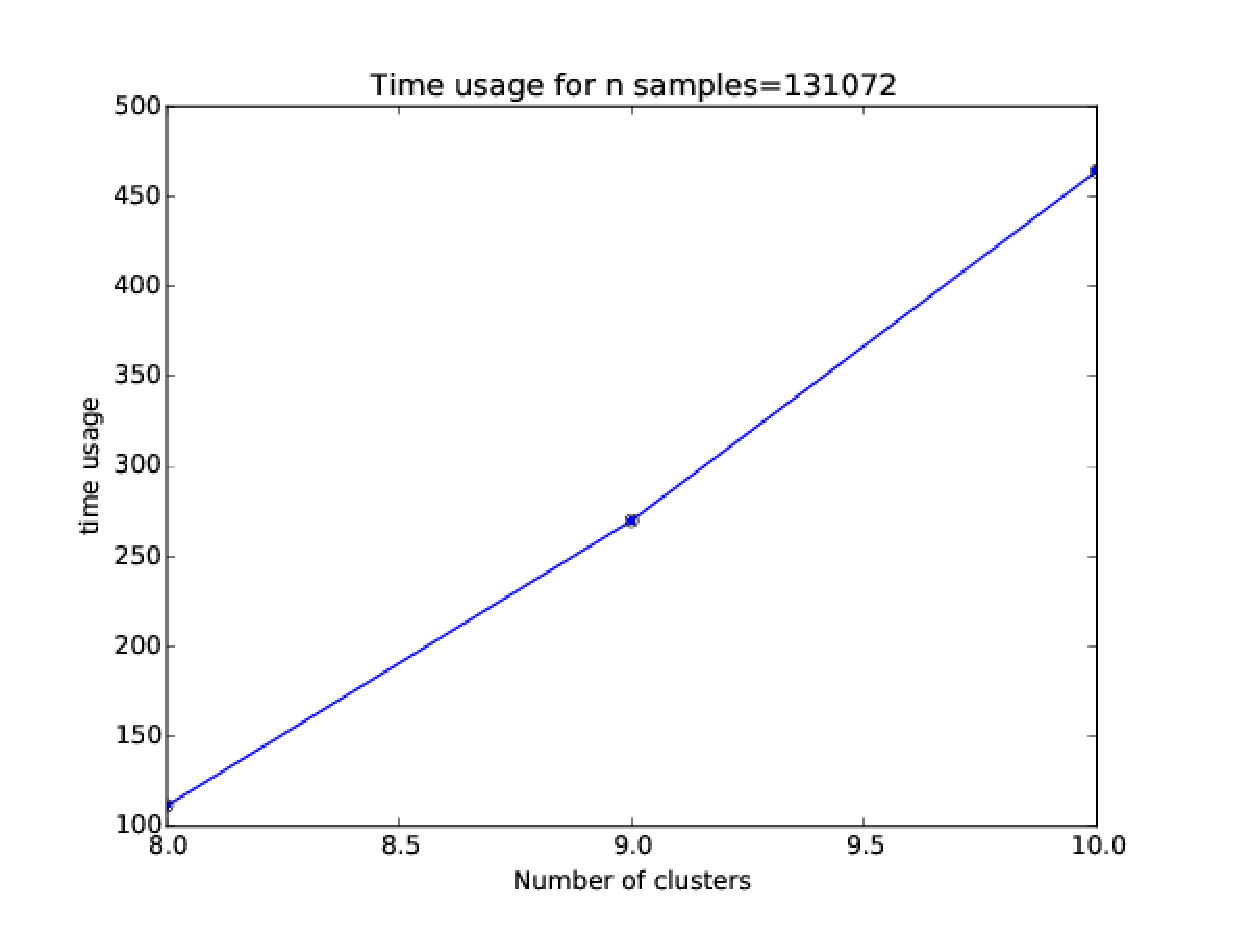
\includegraphics[width=0.60\linewidth]{images/bofwTimeFixedSample}
  \caption{Bag of Words feature representation: Runtime with fixed sample size. (Sample size in $\log_{2}$).  The experiments are run on the actual project dataset.\label{fig:bowf_time_fixed_sample}}
\end{figure}
\begin{figure}
  \centering
  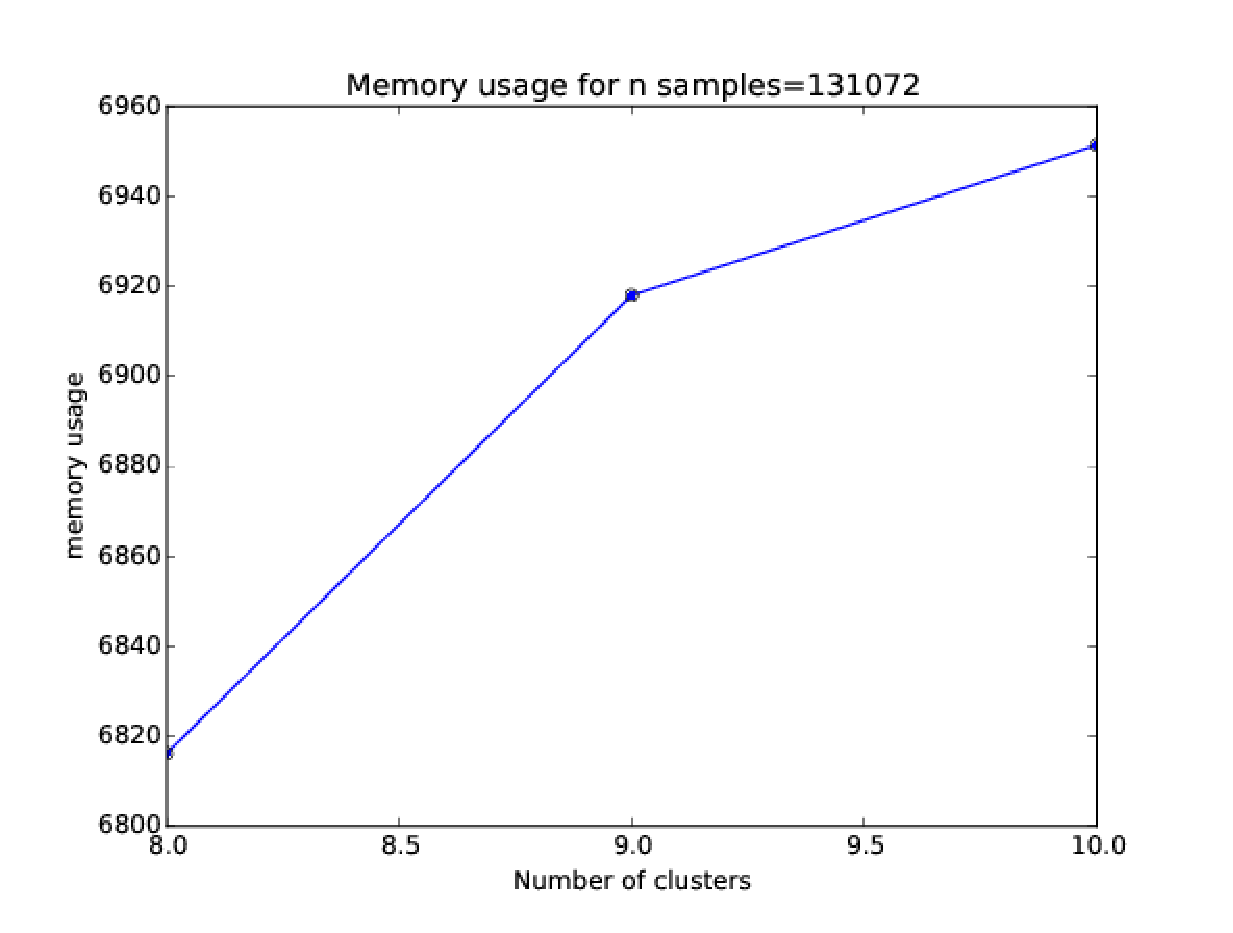
\includegraphics[width=0.60\linewidth]{images/bofwMemoryFixedSample}
  \caption{Bag of Words feature representation: Memory usage with fixed sample size. (Sample size in $\log_{2}$).  The experiments are run on the actual project dataset.\label{fig:bowf_memory_fixed_sample}}
\end{figure}

\subsubsection{Variance Analysis}
We analyze the variance of the Bag of Words representation on a subsample to get an idea of the number of components to use in the downstream pipeline.  A plot of the component vs its variance is displayed in Fig~\ref{fig:bowf_variance}
\begin{figure}
  \centering
  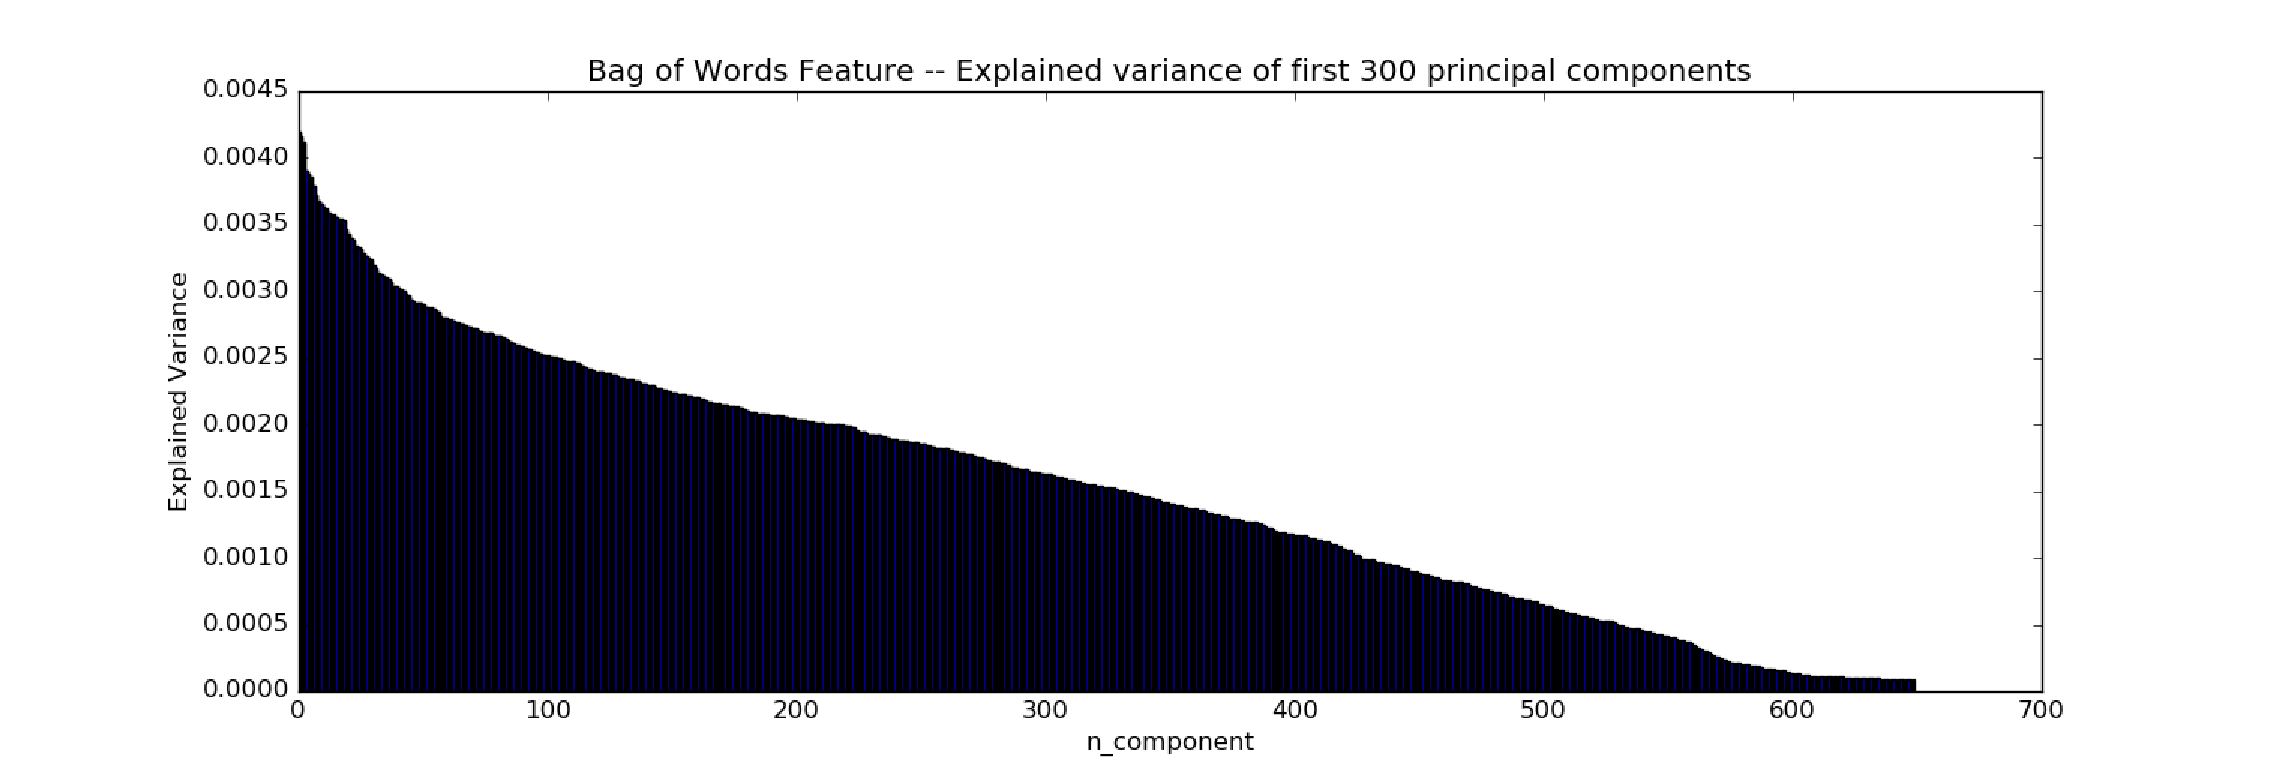
\includegraphics[width=0.75\textwidth]{images/bowf_variance}
  \caption{Explained variance ratio of Bag of Feature representation for a subsample (Subject 1).  We get variance measures of 99, 95, 90, 77, 65 and 50 for components 649, 507, 442, 336, 263, 186 respectively.\label{fig:bowf_variance}} 
\end{figure}


\subsection{Building Vlad model}

\subsubsection{Theory}
Vector of locally aggregated descriptors is a model similar to the Bag of Words model.  
The main difference between BOW and Vlad is that, Vlad takes into account the spread of the information along with the count of local descriptors belonging to a particular centroid.
The vlad representation of a sample with local descriptors of size D and centers K will be given by a matrix of size $K x D $.  Thus a Vlad representation would be able to reperesent more information about the domain than what is capable with a Bow model.

\subsubsection{Algorithm}
The following algorithm enumerates the steps for finding the Vlad representation for a sample with local descriptors.
\begin{enumerate}
  \item Learn the Codebook $ C = \{c_{1}, c_{2} \ldots c_{k}\} $ of words representing the vocabulary of the domain.
  \item Assign the vocabulary for every local descriptor by $ c_{i} = NN(x) $.
  \item The Vlad representation is given by difference $ x - c_{i} $ of the vectors assigned to a particular vocabulary $ c_{i} $.
  \item L2 Normalize the above representation and concatenate the rows to form a vector.
\end{enumerate}

Thus we get the Vlad representation by the simple formula
\begin{align*}
  V_{i,j} = \sum_{x \mid NN(x) = c_{j}} (x_{j} - c_{i, j})
\end{align*}
where $x_{j}$ and $c_{i,j}$ represent the $j^{th}$ component of the descriptor $x$ considered and of its corresponding word $c_{i}$

Thus the Vlad representation of a sample with local desccriptors of dimension D and centers K is given by $ K \times D $.
After concatenating the rows into columns we get a vector of size given by the product of K and D.

\subsubsection{Implementation}
As discussed in the Bag of Words section, since we are using scikit-learn's pipelines, we want to build an implementation that plays nice with scikit learn.  We implemented the fit, transform, set\_params and get\_params method in our vlad implementation.  A brief description of the functions and its operations:
\begin{description}
  \item{def fit (X, Y=None)}  For Vlad implementation: learn the vocabulary of the local descriptors.
  \item{def transform (X)}  Transform a sample containing a list of local descriptors into a vector of dimension K x D (product of cluster size and dimension of local descriptors).
  \item{def set\_params (**params)} Used to set the parameters for grid search.
  \item{def get\_params (deep=True)} Used to get the current parameters.
\end{description}

\subsubsection{Performance}
We try to understand the performance of our Vlad implementation by plotting the runtime and memory usage against a fixed number of clusters.  Fig~\ref{fig:vlad_time_fixed_cluster},~\ref{fig:vlad_memory_fixed_cluster} and also against fixed sample sizes. Refer Fig~\ref{fig:vlad_time_fixed_sample},~\ref{fig:vlad_memory_fixed_sample}.
\begin{figure}
  \centering
  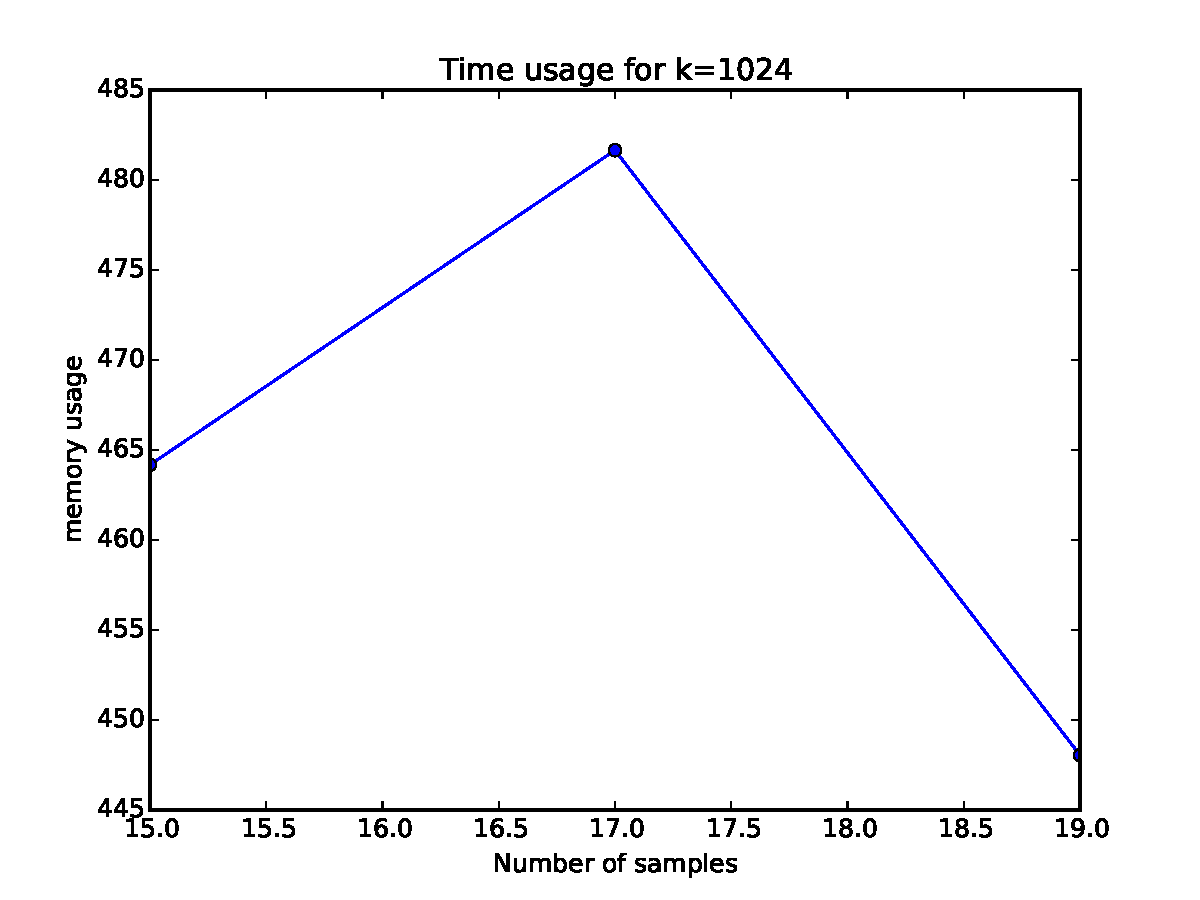
\includegraphics[width=0.60\linewidth]{images/vladTimeFixedCluster}
  \caption{Vlad feature representation: Runtime with fixed cluster size. (Cluster size in $\log_{2}$).  The experiments are run on the actual project dataset.\label{fig:vlad_time_fixed_cluster}}
\end{figure}
\begin{figure}
  \centering
  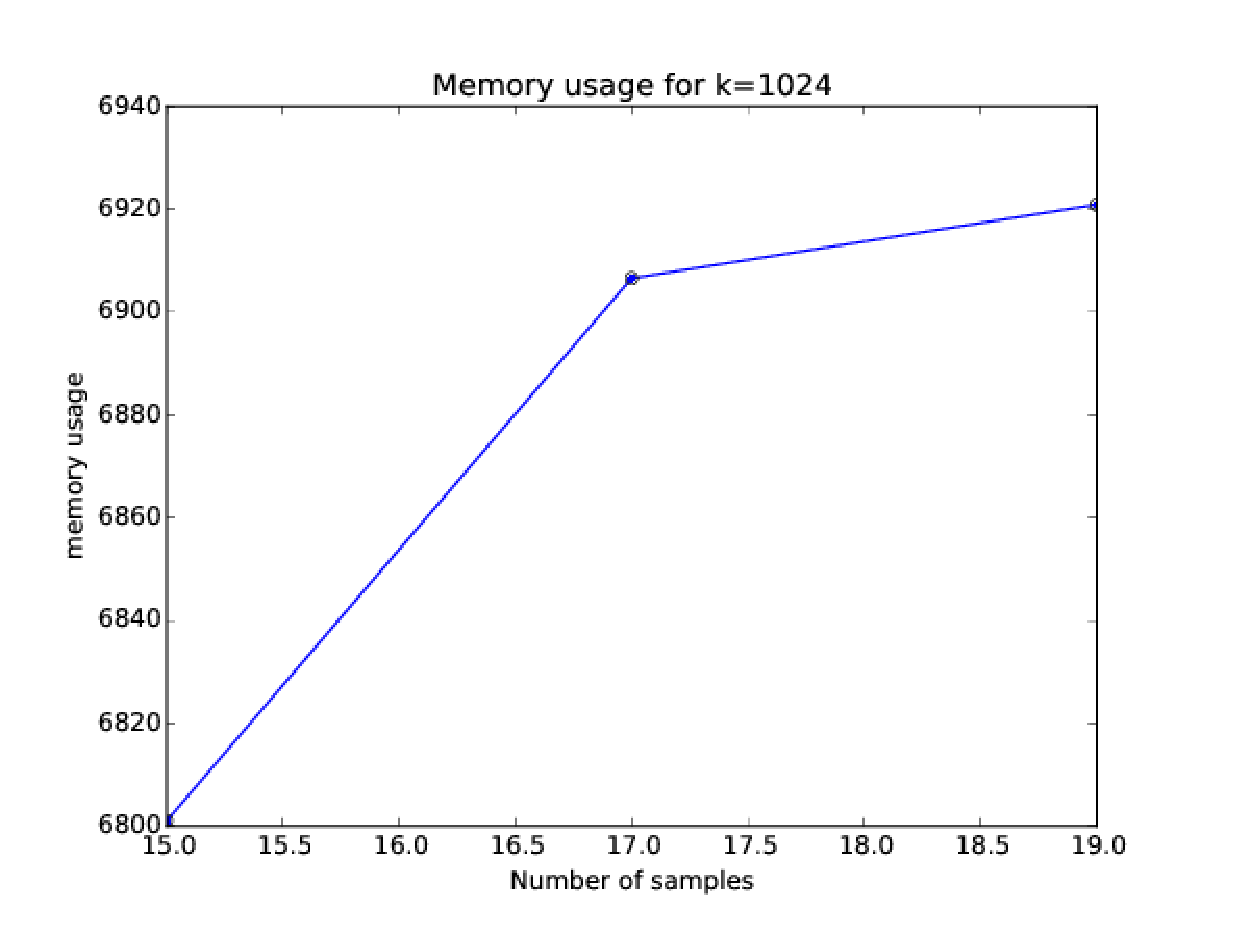
\includegraphics[width=0.60\linewidth]{images/vladMemoryFixedCluster}
  \caption{Vlad feature representation: Memory usage with fixed cluster size. (Cluster size in $\log_{2}$).  The experiments are run on the actual project dataset.\label{fig:vlad_memory_fixed_cluster}}
\end{figure}

\begin{figure}
  \centering
  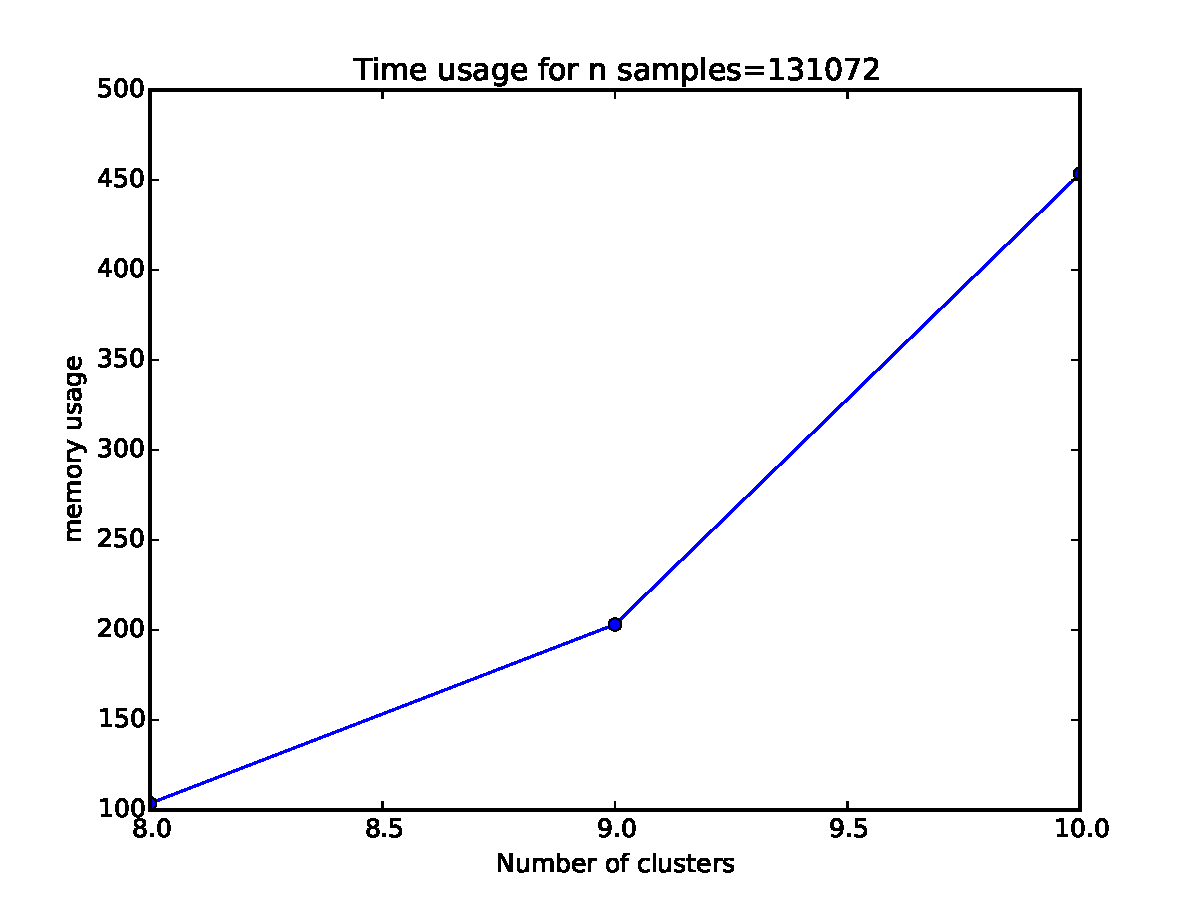
\includegraphics[width=0.60\linewidth]{images/vladTimeFixedSample}
  \caption{Vlad feature representation: Runtime with fixed sample size. (Sample size in $\log_{2}$).  The experiments are run on the actual project dataset.\label{fig:vlad_time_fixed_sample}}
\end{figure}
\begin{figure}
  \centering
  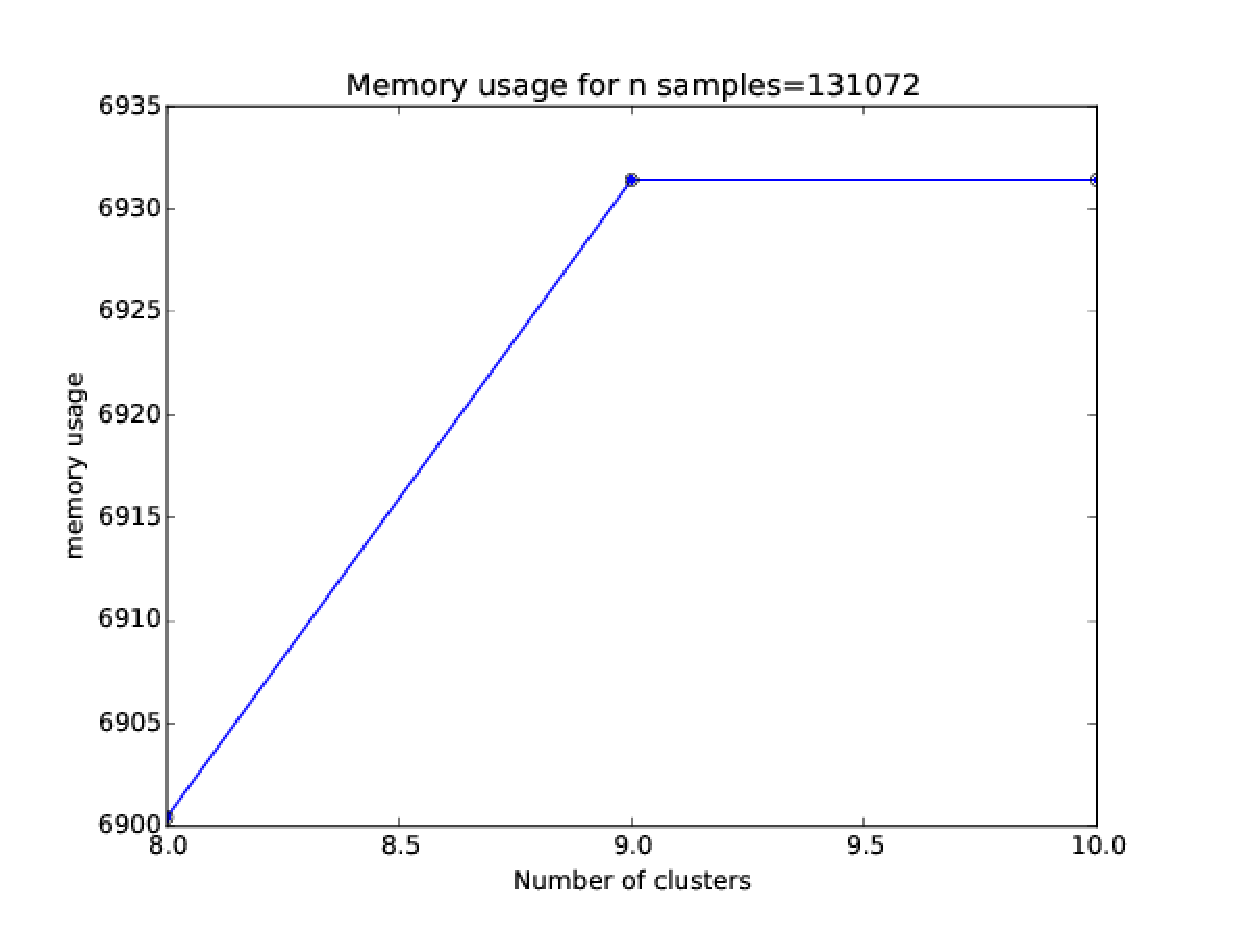
\includegraphics[width=0.60\linewidth]{images/vladMemoryFixedSample}
  \caption{Vlad feature representation: Memory usage with fixed sample size. (Sample size in $\log_{2}$).  The experiments are run on the actual project dataset.\label{fig:vlad_memory_fixed_sample}}
\end{figure}

\subsubsection{Variance Analysis}
We analyze the variance of the Vlad representation on a subsample to get an idea of the number of components to use in the downstream pipeline.  A plot of the component vs its variance is displayed in Fig~\ref{fig:vlad_variance}
\begin{figure}
  \centering
  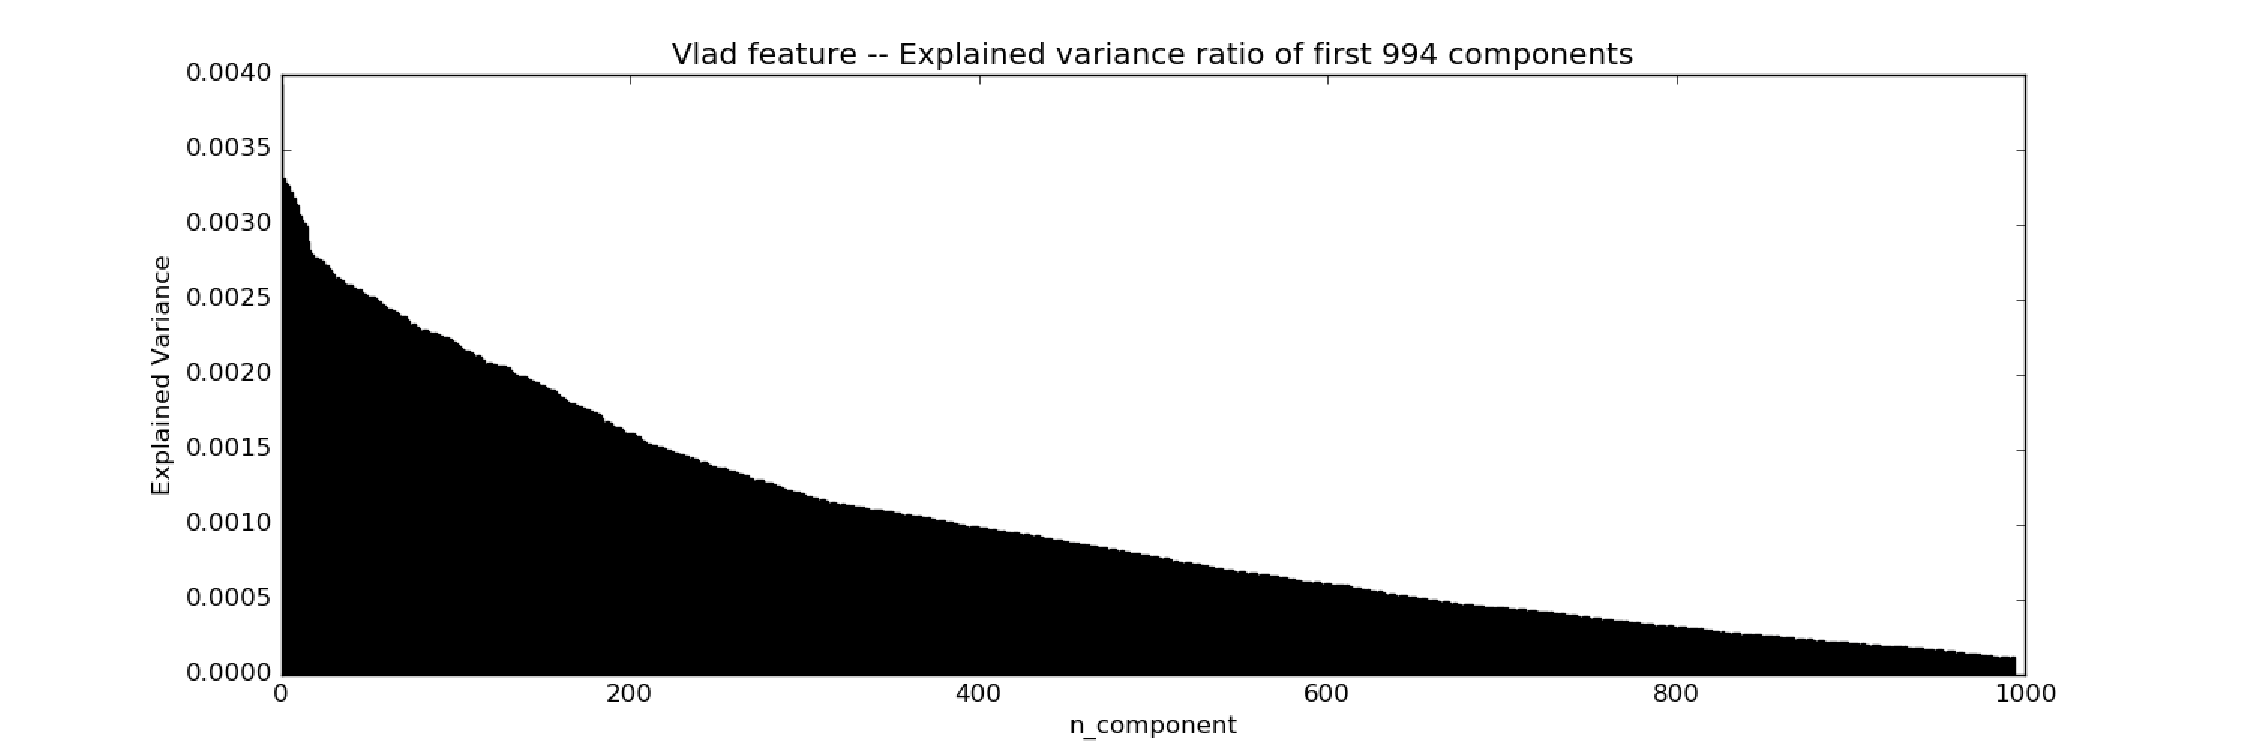
\includegraphics[width=0.75\textwidth]{images/vlad_variance}
  \caption{Explained variance ratio of Vlad representation for a subsample (Subject 1).  We get variance measures of 99, 95, 90, 77, 65 and 50 for components 994, 807, 780, 478, 353, 232 respectively.\label{fig:vlad_variance}} 
\end{figure}


\subsection{Building OnlineMiniBatchKMeans model}
\subsubsection{Theory}
Online Kmeans is a version of the unsupervised KMeans algorithm for clustering huge amount of samples\cite{art:online_kmeans}.  It works similar to Stohastic Gradient Descent but takes batches of samples drawn randomly from the original sample distribution and running KMeans on the subsample.
It is shown that OnlineKMeans has performance comparable to that of KMeans but converges very faster than the originl KMeans algorithm.
\subsubsection{Implementation}
We implemented online kmeans as a component that plays nice with scikit-learn's pipeline.  We also ran a number of experiments with varying cluster sizes to figure out the performance of our algorithm with respect to scikit-learn's KMeans algorithm.
\subsubsection{Performance Optimizations}
We used convergence factor similar to the one used in Scikit-learn's OnlineKMeans to make sure that our algorithm finishes faster.  The performance of our algorithm is very much similar to that of scikit-learn's implementation till sample size --- $2^{17}$ and number of cluster $K = 2^{9}$.
However, since the performance of our pipeline was the best when the cluster size was 1024 or 2048, we are using the Scikit-Learn's implementation in our final version of our code.
Fig~\ref{fig:kmeans_memory} and Fig~\ref{fig:kmeans_time} show the memory and time comparision with respect to scikit-learn.
\begin{figure}
  \centering
  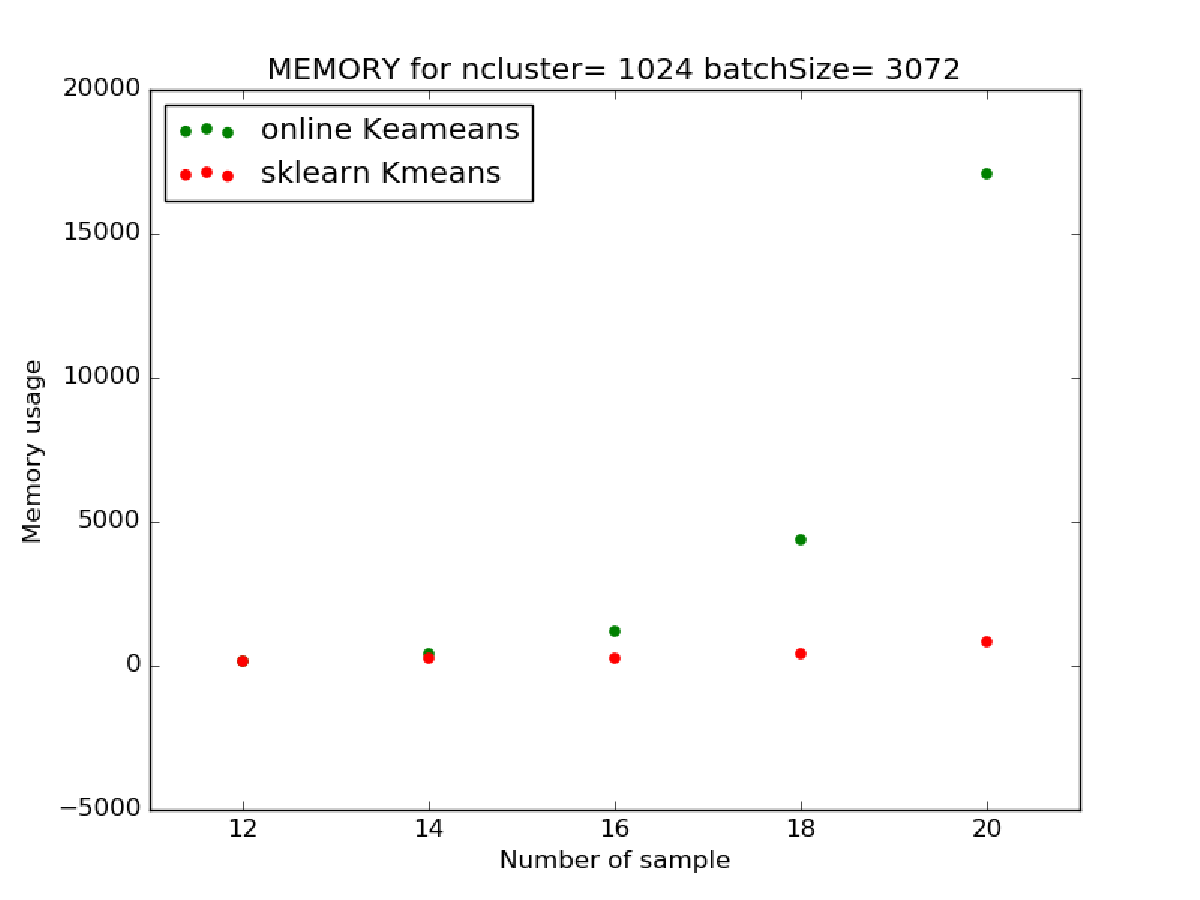
\includegraphics[width=0.75\textwidth]{images/kmeans_memory}
  \caption{Memory usage comparision between custom implementation of KMeans and Scikit-Learn's KMeans algorithm.  Samples are in $\log_{2}$\label{fig:kmeans_memory}} 
\end{figure}
\begin{figure}
  \centering
  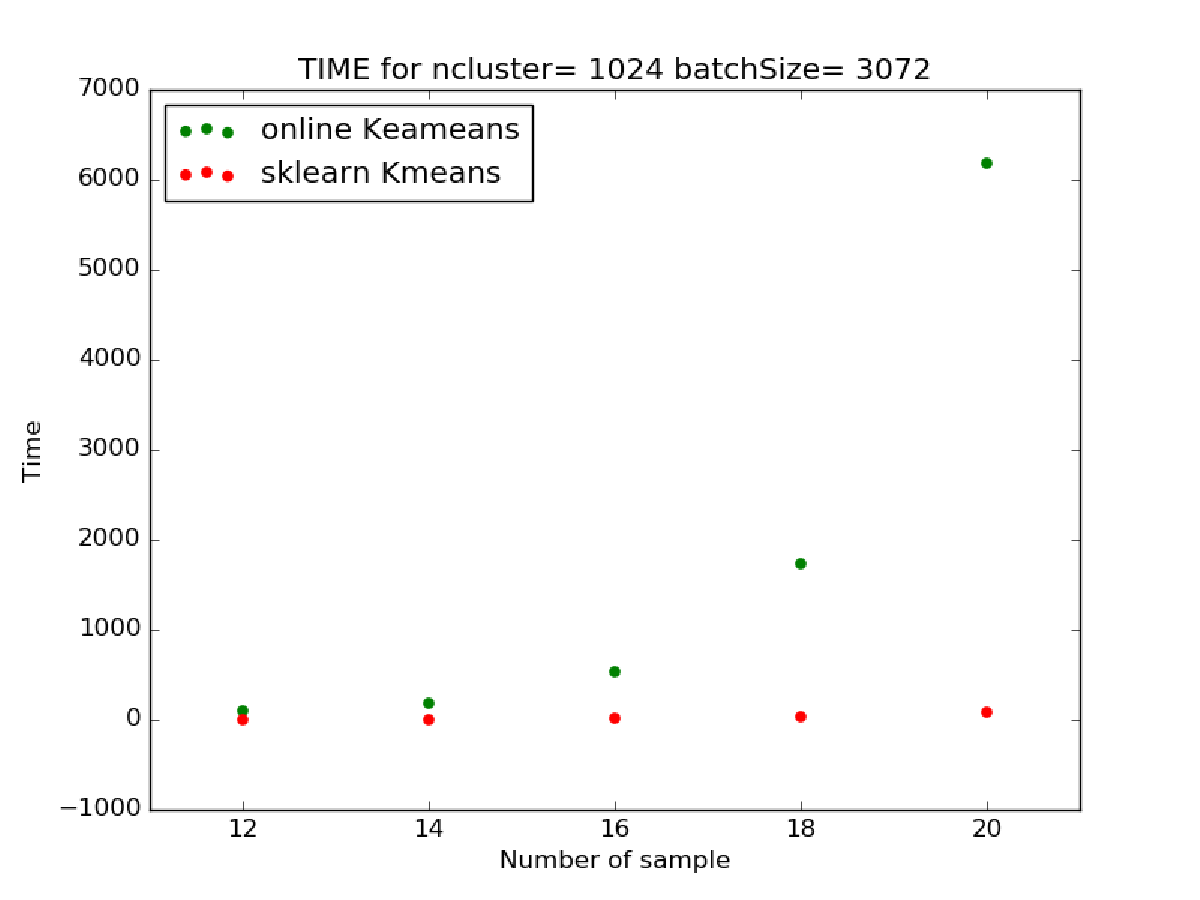
\includegraphics[width=0.75\textwidth]{images/kmeans_time}
  \caption{Runtime comparision between custom implementation of KMeans and Scikit-learn's KMeans algorithm.  Samples are in $\log_{2}$\label{fig:kmeans_time}} 
\end{figure}

\subsection{Putting it all together as a pipeline}
We finally built our pipeline using the following components
  \begin{enumerate}
    \item Preprocessing using xDawn
    \item VLAD / BOW feature representation using our Vlad and Bowf components.
    \item Reduce dimensionality using PCA
    \item Scaling the features using StandardScaler
    \item LinearSVM/GaussianSVM on the scaled feature set
    \item Performance estimation using Mean AUC value.
  \end{enumerate}
\subsection{HyperParameters}
There are a number of hyper parameters which we had to learn for each steps of the pipeline.
\subsubsection{Preprocessing using xDawn}
The value of num\_component is a hyperparameter.  We performed an exhaustive grid search on the pipeline using values of 2, 3 and 4.

Since the data preprocessing takes considerable amount of time, we decided to store the processed values as numpy arrays ans use them in the pipeline downstream.  This saved considerable time for our pipeline.

We were able to observe best performance for num\_component = 2.


\subsubsection{VLAD / BOWF feature representation}
An exhaustive grid search for performed for various values of K ranging from $2^{4}$ to $2^{12}$.
We were able to observe a plateau between K = 1024 and K = 2048.  The best performance was observed for K = 2048, but with K = 4096, the model became computationally intractable.

\subsubsection{PCA}
We reduced the dimension of the feature set to 90\% of the explained variance of the original dataset.

\subsubsection{LinearSVM and GaussianSVM}
We ran exhaustive grid search for values of C and Gamma ranging from $2^{-4}$ to $2^{4}$.

\section{Results and Analysis}
This section contains the results and analysis of our results.  We will plot the results for a few cases of grid search, performance, and accuracy score.
\subsection{Best Performance}
We got the best performance of 0.52 misclassification score with Linear SVM and Bowf representation for parameters
\begin{enumerate}
  \item  xDawn --- num\_component = 2
  \item  Bowf --- Cluster size (K) = 2048
  \item  classifier --- LinearSVM
  \item  Classifier parameters --- C = 16.000
\end{enumerate}

\subsection{ROC curves}
The performance criteria we used is the mean ROC curve.  
Fig~\ref{fig:roc_hpc} and Fig~\ref{fig:roc_mean} shows the mean ROC curve and actual ROC curve for all the stimulus.
\begin{figure}
  \centering
  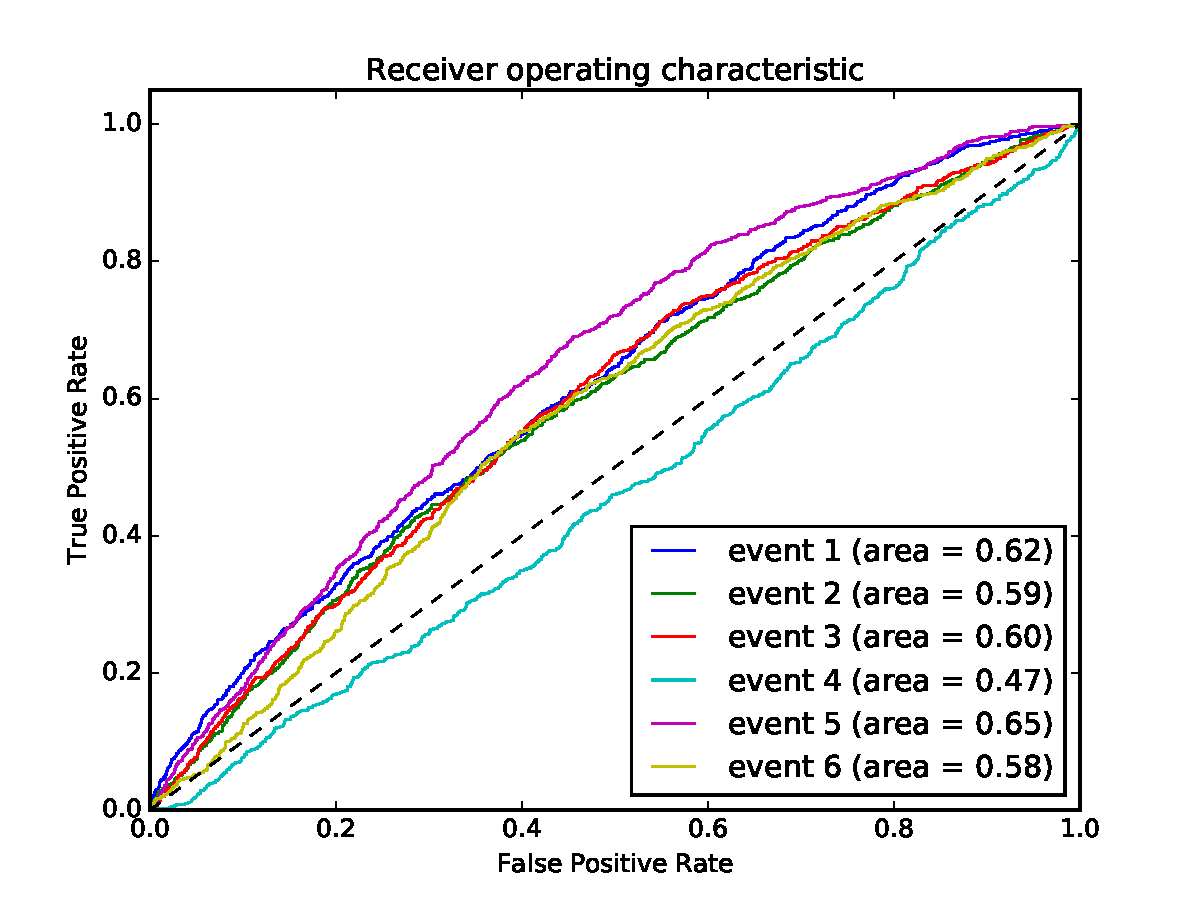
\includegraphics[width=0.60\linewidth]{images/ROC6Partials}
  \caption{ROC Partials (n\_components=2,C=4,n\_culter=2**8).\label{fig:roc_hpc}}
\end{figure}
\begin{figure}
  \centering
  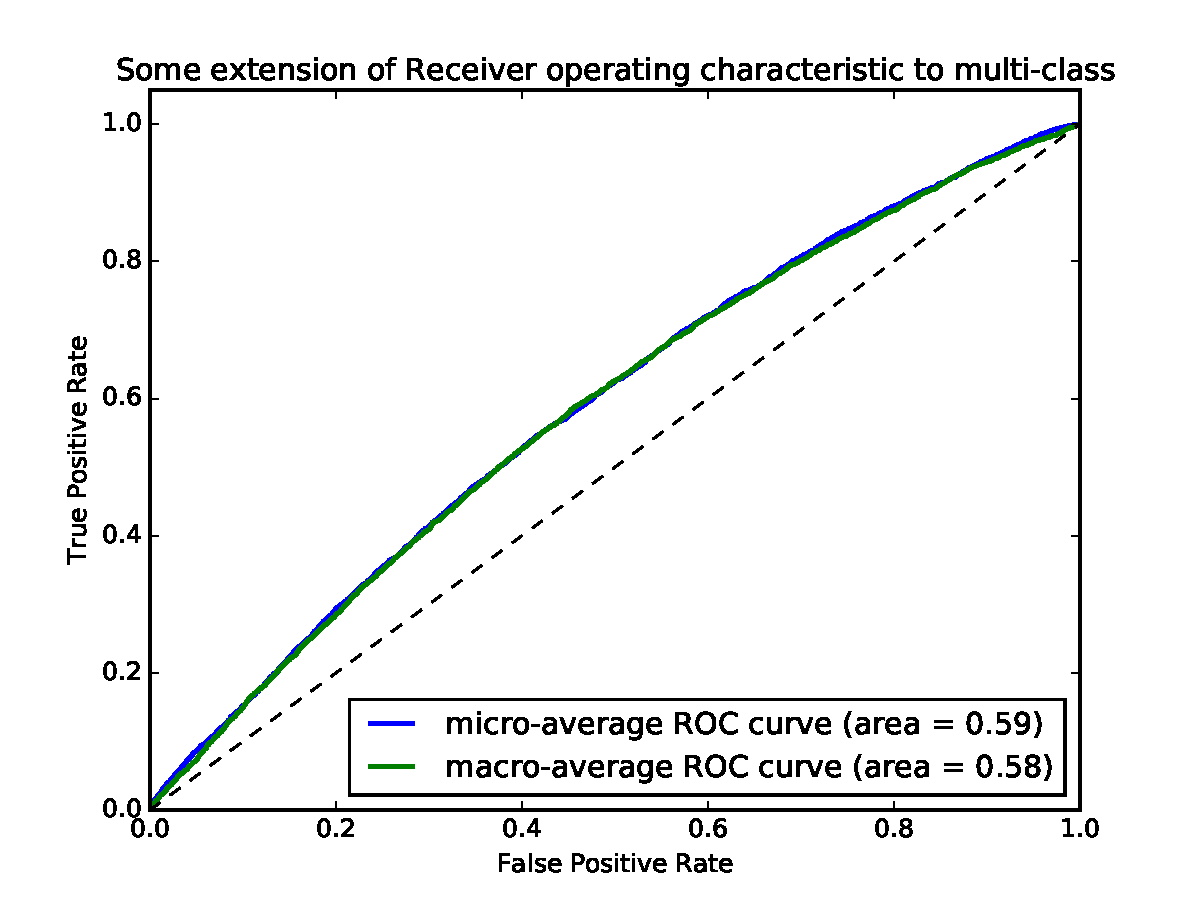
\includegraphics[width=0.60\linewidth]{images/ROCMean}
  \caption{Mean ROC curve (n\_components=2,C=4,n\_culter=2**8).\label{fig:roc_mean}}
\end{figure}

\subsection{Grid Search}
The plots Fig~\ref{fig:bowf_score2} and Fig~\ref{fig:bowf_score3} shows the accuracy of the cross validation scripts with respect to C values.  
Note that the accuracy in the plot is with respect to the misclassification error and not the Area Under the Curve.

A sample run of the cross validation with top ten scores is shown in Table~\ref{2compTable}
\begin{table}[]\label{2compTable}
\centering
\caption{Bag of words score for xDawn num\_component$=2$}
\label{2comp}
\begin{tabular}{lllll}
  C      &    K &    Score &       Time \\  
16.0000 & 2048 & 0.531901 & 317.500000  \\
8.0000  & 2048 & 0.530237 & 196.500000  \\                                                                            
4.0000  & 2048 & 0.516204 & 173.500000  \\                                                                            
2.0000  & 2048 & 0.501374 & 132.000000  \\  
1.0000  & 2048 & 0.491392 &  95.733333  \\                                                                            
0.5000  & 2048 & 0.474392 &  84.800000  \\                                                                            
0.2500  & 2048 & 0.461661 &  59.866667  \\                                                                            
0.1250  & 2048 & 0.442564 &  67.966667  \\                                                                            
0.0625  & 2048 & 0.430555 &  48.066667  \\                                                                            
16.0000 & 1024 & 0.358941 & 475.833333  \\                                                                            
\end{tabular}
\end{table}

\begin{figure}
  \centering
  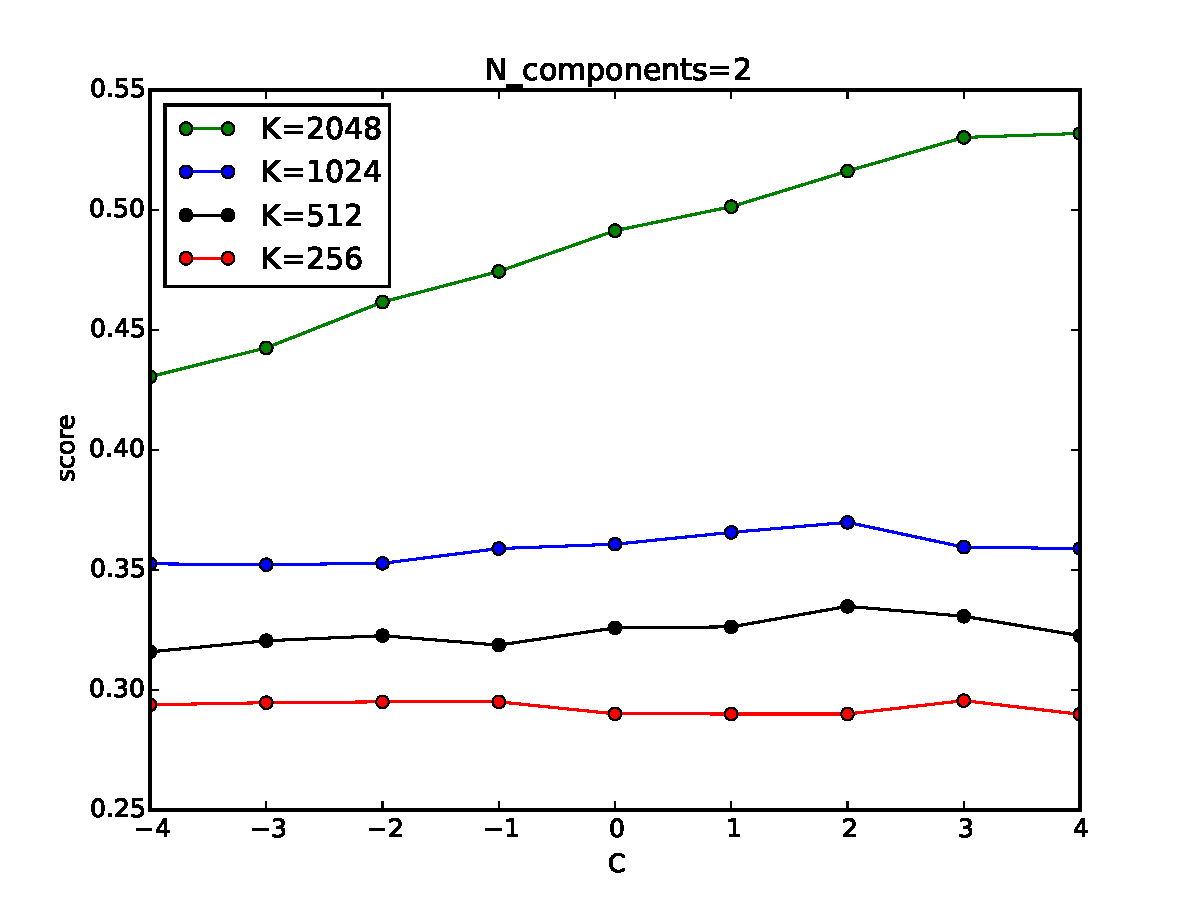
\includegraphics[width=0.60\linewidth]{images/score2Components}
  \caption{The C vs score plot for Linear Bow features. When n\_components = 2.  The maximum score is obtained for C=4.\label{fig:bowf_score2}}
\end{figure}

\begin{figure}
  \centering
  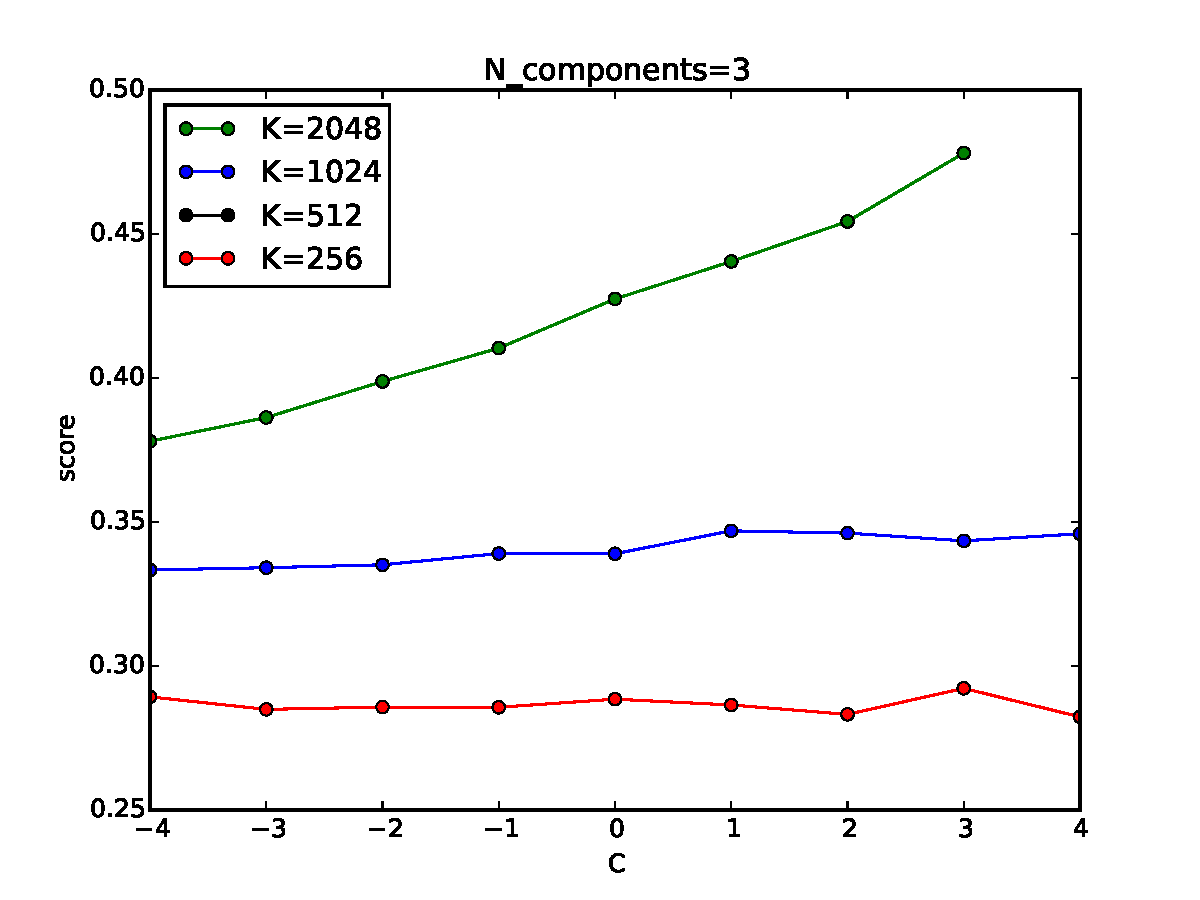
\includegraphics[width=0.60\linewidth]{images/score3Components}
  \caption{The C vs score plot for Linear Bow feature When n\_components = 3.  For K=2048, the computation became intractable.  So we dont have any datapoint for K=2048 and $C=2^{4}$\label{fig:bowf_score3}}
\end{figure}

\subsection{Performance}
The plots Fig~\ref{fig:bowf_time2} and Fig~\ref{fig:bowf_time3} shows the time usage of the cross validation scripts with respect to C values.
\begin{figure}
  \centering
  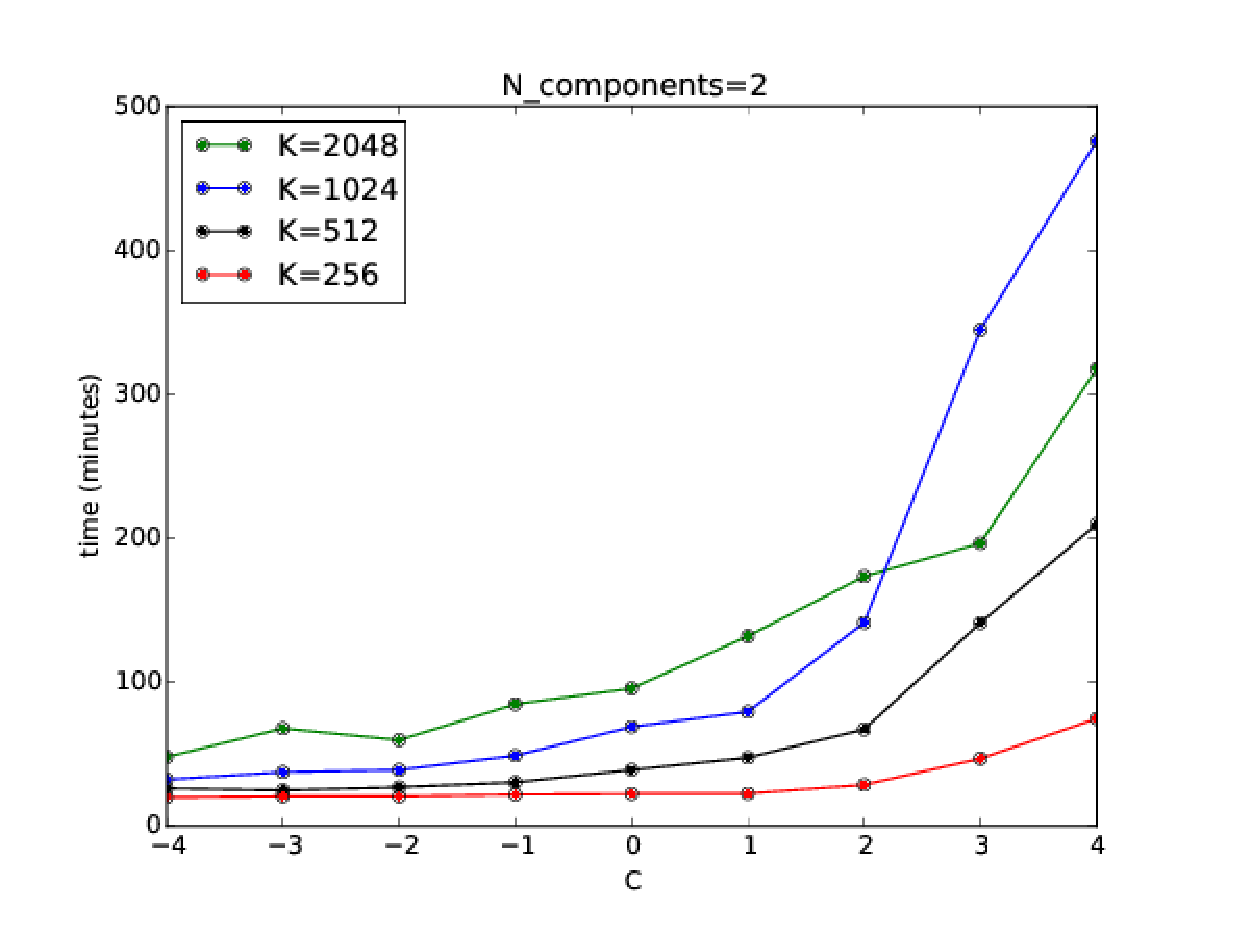
\includegraphics[width=0.60\linewidth]{images/time2Components}
  \caption{The C vs time plot for Linear Bow features. When n\_components = 2.  The jump for K=1024 after log2(C)=2 made us curious.  We are not exactly sure about what causes the jump.\label{fig:bowf_time2}}
\end{figure}

\begin{figure}
  \centering
  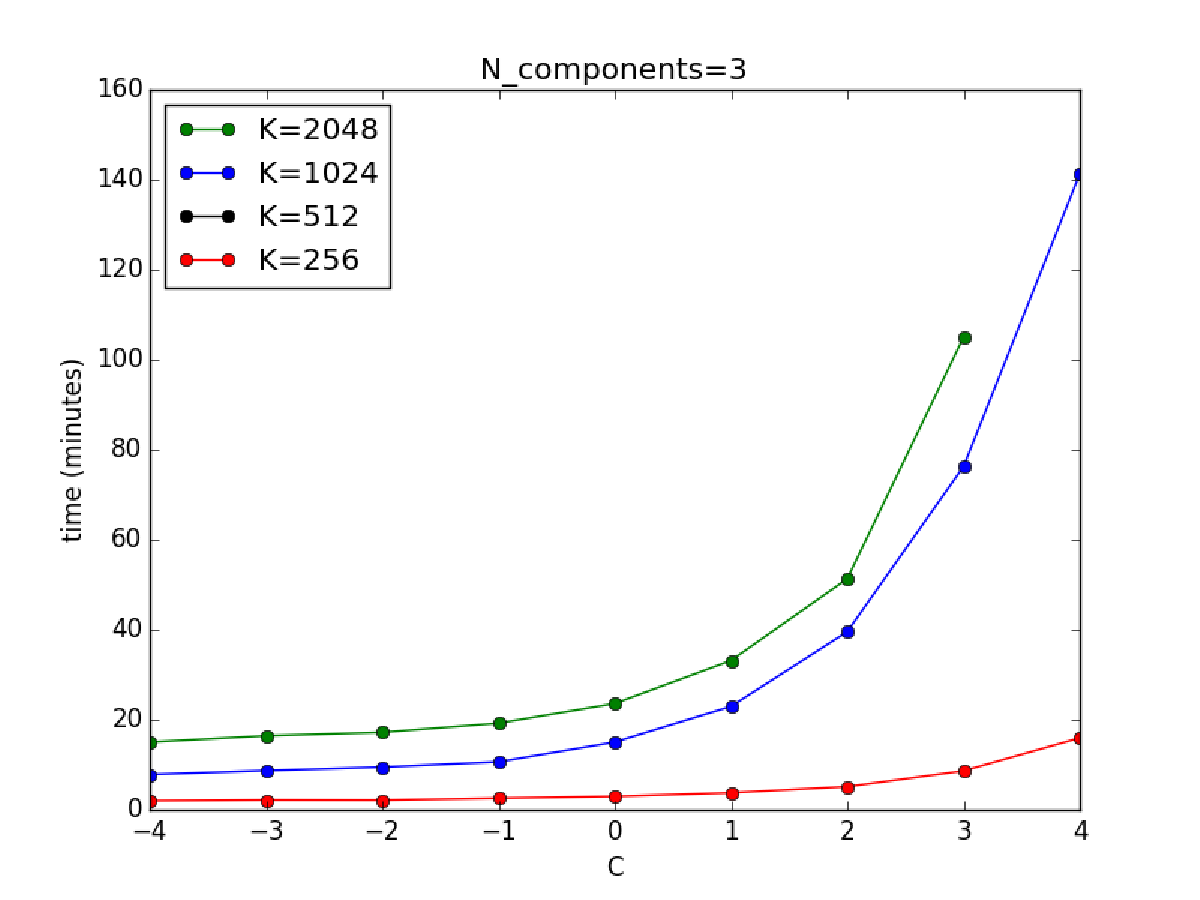
\includegraphics[width=0.60\linewidth]{images/time3Components}
  \caption{The C vs time plot for Linear Bow feature When n\_components = 3.  We were unable to get a datpoint for K=2048 and log2(C)=4 as the computation took more than 30 hours and still didn't finish.\label{fig:bowf_time3}}
\end{figure}


\section{Future work and Potential Improvements}
\subsection{Feature Selection}
  On analysing the performance and the choice of features retrospectively, we are able to realize that using just xDawn filters for feature selection might not be a good decision.  
The baseline uses Linear Discriminant Analysis and a set of Filter Bank along with xDawn for its feature selection.
The current Vlad and Bowf model should be trained again by using a better feature set to understand the performance difference.

Also, a spatial analysis of the EEG signals with respect to the location of electrodes and analysing the evoked potentials with respect to a particular stimulus whould have given a better understanding of the input data.

The models used in this project should give a much better performance if proper care is taken to select the feature set properly.

\subsection{Pipeline}
Though we did a grid search on a number of parameters such as C, Gamma, num\_components, and K\@; we didn't do grid search on the dimensionality reduction.  
This was based on the assumption that for best results the reduced data should still hold the maximum amount of variance.
Performing grid search on the number of reduced components such that the variance is at 50, 65, 77, 90, 95 and 99 percentile of the orignal variancce would have given better results.

Also, we were unable to run our experiments to get a peak in the plots for all the hyperparameters.  
The performance was increasing for values of K=2048 and C=16.  
But we were unable to run more number of jobs as the jobs were taking more than 30 hours.  
A considerable time should be spent to optimize the Vlad/Bowf implementation further before running the implementation.


\subsection{Process}
We did a lot of analysis such as the separability of the dataset, variance of the features, characteristics of the raw data retrospectively.  If these analysis were done before starting up with the pipeline, we might have got better feature representations.

\subsection{No future data rule}
The current implementation does't abide by the no future data rule.  We should find ways to abide by the no future data rule and get good accuracy predictions.


\section{Code and Plots}
The complete codebase, HPC job outputs, and original plots are all available at our Github repository.\cite{repo:github}

\section{Hardware Requirements}
The huge size of the dataset requires that we use systems with high capacity.  Almost all our jobs in HPC were run with the following specs:
\begin{description}
  \item{CPU Cores:}  12 core.
  \item{CPU Nodes:}  1 Node.
  \item{RAM:}  164 GB\@.
  \item{Runtime:} Minimum 24 hours.  (Jobs with >= 2048 clusters got killed even after 30 hours.)
  \item{GPU:} None
\end{description}

\section{Acknowledgements}
We would like to thank our Professor Zaid Harchaoui for being helpful all the time and guiding us throughout the project. 
Many thanks to the authors of the baseline implementation who helped us in understanding the preprocessing steps and also helped us through emails
whenever we got struck.

Thanks to the NYU HPC team for promptly resolving any issues we had with the HPC Clusters.

\newpage

\bibliographystyle{siam}
\bibliography{references}

\end{document}
